\documentclass[12pt,a4paper]{article}

% =============================================================================
% PACKAGES
% =============================================================================
\usepackage[utf8]{inputenc}
\usepackage[T1]{fontenc}
\usepackage{amsmath,amssymb,amsthm}
\usepackage{mathtools}
\usepackage{booktabs}
\usepackage{array}
\usepackage{tabularx}
\usepackage{graphicx}
\usepackage{tikz}
\usetikzlibrary{shapes,arrows,positioning}
\usepackage[dvipsnames]{xcolor}
\usepackage{tcolorbox}
\tcbuselibrary{theorems,skins,breakable}
\usepackage{enumitem}
\usepackage{geometry}
\geometry{margin=2.5cm}
\usepackage{setspace}
\onehalfspacing
\usepackage{natbib}
\bibliographystyle{apalike}
\usepackage{hyperref}
\hypersetup{
    colorlinks=true,
    linkcolor=blue,
    citecolor=blue,
    urlcolor=blue
}

% =============================================================================
% CUSTOM COMMANDS
% =============================================================================
\newcommand{\GTWH}{\textsc{gtwh}}

% =============================================================================
% TITLE
% =============================================================================
\title{
\vspace{-2cm}
\textbf{\LARGE The General Theory of Welfare Hierarchies}\\[0.5em]
\large A Unified Framework for Multi-Level Welfare Analysis
}

\author{
\textbf{Gerhard Fehr}\thanks{Corresponding author. Email: gerhard.fehr@fehradvice.com}\\
FehrAdvice \& Partners AG, Zürich\\[0.5em]
\textbf{Andrea Fehr}\\
FehrAdvice \& Partners AG, Zürich
}

\date{January 2026\\[1em]
\small Working Paper}

% =============================================================================
% DOCUMENT
% =============================================================================
\begin{document}

\maketitle

\begin{abstract}
\noindent
We present the \textbf{General Theory of Welfare Hierarchies (GTWH)}, a unified 
framework that resolves the fundamental aggregation problem in welfare economics. 
The theory derives the complete structure of social levels---from individual to 
humanity---from first principles, showing that levels are \emph{endogenously 
defined} by shared identity (IDN) and collective utility (KNU) rather than 
exogenously assumed. The framework features: (1) a recursive, self-similar 
utility structure that applies identically at every level; (2) three formally 
specified inter-level dynamics (upward aggregation, downward causation, 
horizontal spillover); (3) a cross-level complementarity matrix capturing 
how levels reinforce or undermine each other; and (4) context-dependent 
level salience determined by the environment. The theory unifies methodological 
individualism with holistic approaches, bridges micro and macro analysis, 
and provides a rigorous foundation for welfare economics, social choice theory, 
and policy design across all scales of human organization.

\vspace{1em}
\noindent\textbf{Keywords:} Welfare economics, aggregation problem, multi-level 
analysis, social hierarchy, utility theory, complementarity, identity economics

\noindent\textbf{JEL Classification:} D60, D71, D91, Z13
\end{abstract}

\newpage
\tableofcontents
\newpage

%%%%%%%%%%%%%%%%%%%%%%%%%%%%%%%%%%%%%%%%%%%%%%%%%%%%%%%%%%%%%%%%%%%%%%%%%%%%%%%
\section{Introduction: The Aggregation Problem}
\label{sec:introduction}
%%%%%%%%%%%%%%%%%%%%%%%%%%%%%%%%%%%%%%%%%%%%%%%%%%%%%%%%%%%%%%%%%%%%%%%%%%%%%%%

\subsection{The Central Problem of Welfare Economics}

Since Arrow's (1951) impossibility theorem, welfare economics has struggled 
with a fundamental question: \textit{How do individual utilities aggregate to 
social welfare?} The problem is not merely technical but conceptual:

\begin{itemize}[nosep]
\item What is the relationship between individual and collective welfare?
\item Do groups, organizations, and nations have welfare beyond their members?
\item How do we compare welfare across different levels of social organization?
\item Why do policies that help individuals sometimes harm communities, and vice versa?
\end{itemize}

\subsection{The Limitations of Existing Approaches}

Current approaches fall into two camps, each with fundamental limitations:

\begin{enumerate}[nosep]
\item \textbf{Methodological Individualism}: Only individuals have utility; 
social welfare is merely the sum of individual utilities. 
\textit{Problem}: Cannot explain why tribal identity affects behavior, 
why national institutions matter, or why communities have emergent properties.

\item \textbf{Holistic Approaches}: Groups have irreducible properties that 
cannot be explained by individual behavior.
\textit{Problem}: No micro-foundation; cannot explain how group properties 
emerge from individual actions.
\end{enumerate}

\subsection{The GTWH Resolution}

The General Theory of Welfare Hierarchies resolves this tension by showing that:
\begin{enumerate}[nosep]
\item Levels are \textbf{endogenously defined} by shared identity and collective structure
\item The \textbf{same utility formula} applies at every level (self-similarity)
\item Levels \textbf{interact dynamically} through upward, downward, and horizontal connections
\item Level \textbf{salience depends on context}, explaining situational variation
\item The framework \textbf{converges} to a well-defined meta-level (all sentient beings)
\end{enumerate}

%%%%%%%%%%%%%%%%%%%%%%%%%%%%%%%%%%%%%%%%%%%%%%%%%%%%%%%%%%%%%%%%%%%%%%%%%%%%%%%
\section{The Core Insight: Endogenous Levels}
\label{sec:core-insight}
%%%%%%%%%%%%%%%%%%%%%%%%%%%%%%%%%%%%%%%%%%%%%%%%%%%%%%%%%%%%%%%%%%%%%%%%%%%%%%%

\subsection{The Conventional View}

Standard economics assumes levels exist exogenously:
\begin{itemize}[nosep]
\item Microeconomics: Individuals and firms (given)
\item Macroeconomics: Nations and economies (given)
\item International economics: Countries (given)
\end{itemize}

The levels are simply \textit{assumed}, not derived.

\subsection{The GTWH Innovation}

We reverse the logic. Instead of assuming levels and asking how they interact, 
we ask: \textit{What defines a level?}

\begin{tcolorbox}[colback=blue!5!white, colframe=blue!75!black, title=The Endogeneity Principle]
\textbf{A level exists if and only if there is shared identity (IDN) or 
shared collective utility (KNU).}

\begin{equation}
\boxed{
\text{Level } L \text{ exists} \iff \exists \, IDN^L \text{ (shared identity)} \lor \exists \, KNU^L \text{ (shared collective)}
}
\label{eq:endogeneity}
\end{equation}

Levels are not given---they are \textbf{created} by human identification and cooperation.
As Fehr and Fischbacher (2003) demonstrate, human cooperation extends far beyond 
kin and reciprocal relationships---a ``nature of human altruism'' that enables 
the formation of large-scale cooperative structures (levels) among genetically 
unrelated individuals. Critically, Fehr, Fischbacher, and Gächter (2002) show 
that this cooperation is sustained by ``strong reciprocity''---a behavioral 
propensity that cannot be explained by standard evolutionary theories (kin 
selection, reciprocal altruism) but is consistent with \textbf{multilevel 
selection and cultural evolution}. More recently, Fehr and Schurtenberger (2018) 
provide comprehensive evidence that \textbf{social norms are causal drivers of 
human cooperation}, with the norm of conditional cooperation explaining major 
cooperation-related regularities across societies. This provides the evolutionary 
and normative foundation for why welfare hierarchies emerge and persist: 
cooperation at multiple levels is not just individually rational but 
evolutionarily and normatively stable.
\end{tcolorbox}

\subsection{Implications of Endogenous Levels}

\begin{itemize}[nosep]
\item \textbf{Levels can emerge}: When people form a shared identity (``We are X''), 
a new level comes into existence.
\item \textbf{Levels can dissolve}: When identity fades or collectives fragment, 
levels disappear.
\item \textbf{Levels are context-dependent}: The same person belongs to multiple 
levels; which is salient depends on context.
\item \textbf{Levels are empirically identifiable}: Wherever we find shared 
identity or collective structure, there is a level.
\end{itemize}

%%%%%%%%%%%%%%%%%%%%%%%%%%%%%%%%%%%%%%%%%%%%%%%%%%%%%%%%%%%%%%%%%%%%%%%%%%%%%%%
\section{The Foundational Structure}
\label{sec:foundation}
%%%%%%%%%%%%%%%%%%%%%%%%%%%%%%%%%%%%%%%%%%%%%%%%%%%%%%%%%%%%%%%%%%%%%%%%%%%%%%%

\subsection{The Meta Level: The Ultimate Scope}

\subsubsection{The Foundational Question}

Before deriving levels, we must answer: \textit{What is the ultimate scope of 
welfare analysis?}

\subsubsection{The Sentience Criterion}

Following Nagel (1974), Chalmers (1996), and Singer (1975), we 
adopt the principle that welfare requires a \textit{subject of experience}---an 
entity for which there is ``something it is like'' to be that entity. Chalmers' 
formulation of the ``hard problem of consciousness'' provides the philosophical 
foundation: subjective experience (qualia) cannot be reduced to functional or 
physical descriptions, yet it is precisely this subjective dimension that makes 
welfare possible. An entity without phenomenal consciousness---without 
``something it is like'' to be that entity---cannot have welfare in any 
meaningful sense.

\begin{tcolorbox}[colback=green!5!white, colframe=green!50!black, title=Definition: The Meta Level]
\begin{equation}
\boxed{
U^{Meta} = \int_{t=0}^{\infty} \sum_{i \in S_t} \delta^t \cdot U^i_t \, dt
}
\label{eq:meta-level}
\end{equation}

where $S_t$ is the set of all sentient beings at time $t$, and $\delta$ is the 
intergenerational discount factor.

The Meta level encompasses \textbf{all welfare that exists or will exist}.
\end{tcolorbox}

\subsubsection{Philosophical Grounding}

This formulation:
\begin{itemize}[nosep]
\item Includes all humans (present and future)
\item Includes sentient animals (per Singer's expanding circle)
\item Potentially includes future artificial sentience
\item Provides a well-defined upper bound for the hierarchy
\end{itemize}

\subsection{The Recursive Structure}

\subsubsection{The Self-Similarity Principle}

A remarkable feature of welfare hierarchies is their \textit{self-similarity}: 
the same mathematical structure applies at every level.

\begin{tcolorbox}[colback=yellow!5!white, colframe=yellow!50!black, title=The Recursive Welfare Formula]
At \textbf{any} level $L$:

\begin{equation}
\boxed{
U^L_{d,t}(\Psi) = \left(\delta^L_d(\Psi)\right)^t \cdot \left[ G^L_{d,t} - \lambda^L_d(\Psi) \cdot P^L_{d,t} \right]
}
\label{eq:recursive-utility}
\end{equation}

\textbf{Aggregation} from level $L-1$ to level $L$:

\begin{equation}
\boxed{
U^L = \sum_{i \in M^L} \omega^L_i \cdot U^{L-1}_i + \sum_{i < j} \gamma^L_{ij} \cdot U^{L-1}_i \cdot U^{L-1}_j
}
\label{eq:aggregation}
\end{equation}

The formula is \textbf{fractal}: zoom in or out, and you see the same structure.
\end{tcolorbox}

\subsubsection{Why Self-Similarity?}

The self-similar structure is not arbitrary. It reflects:
\begin{itemize}[nosep]
\item \textbf{Prospect theory} (Kahneman \& Tversky, 1979): Gain-loss asymmetry 
operates at all levels---individuals fear losses, so do organizations and nations.
\item \textbf{Social preferences} (Fehr \& Schmidt, 1999): Inequality aversion 
and fairness concerns operate at individual, group, and societal levels.
\item \textbf{Discounting} (Samuelson, 1937): All entities discount the future, 
whether persons, firms, or governments.
\item \textbf{Complementarity} (Milgrom \& Roberts, 1990): Interaction effects 
exist at every level of organization.
\item \textbf{Cooperation and punishment} (Fehr \& Gächter, 2000, 2002): The 
mechanisms sustaining cooperation---including altruistic punishment---operate 
analogously at all levels of social organization.
\item \textbf{Super-additive cooperation} (Efferson, Bernhard, Fischbacher \& Fehr, 2024): 
Neither repeated interactions nor intergroup competition alone can reliably sustain 
cooperation---but combining both mechanisms produces ``super-additive'' effects. 
This directly supports GTWH's core insight that \textit{multiple levels interact} 
to produce stable cooperation.
\end{itemize}

%%%%%%%%%%%%%%%%%%%%%%%%%%%%%%%%%%%%%%%%%%%%%%%%%%%%%%%%%%%%%%%%%%%%%%%%%%%%%%%
\section{The Level Hierarchy}
\label{sec:hierarchy}
%%%%%%%%%%%%%%%%%%%%%%%%%%%%%%%%%%%%%%%%%%%%%%%%%%%%%%%%%%%%%%%%%%%%%%%%%%%%%%%

\subsection{Derived Levels}

Applying the endogeneity principle, we derive the following hierarchy:

\begin{table}[htbp]
\centering
\caption{The GTWH Level Hierarchy}
\label{tab:hierarchy}
\renewcommand{\arraystretch}{1.3}
\begin{tabular}{@{}clll@{}}
\toprule
$L$ & \textbf{Level} & \textbf{Defining Condition} & \textbf{Examples} \\
\midrule
0 & Individual & Sentience (base case) & A person \\
1 & Primary Group & Kinship, strong bonds & Family, close friends \\
2 & Tribe/Community & Shared identity ``We are X'' & Profession, village, clan \\
3 & Organization & Formal collective structure & Firm, party, church \\
4 & Network & Functional interdependence & Industry, movement \\
5 & Region & Geographic collective & City, state, canton \\
6 & Nation & Political collective & Country \\
7 & Supranational & Treaty-based collective & EU, ASEAN \\
8 & Species & Biological identity & Humanity \\
9 & Sentient & Consciousness & All sentient beings \\
$\infty$ & Meta & Intertemporal & All sentient, all time \\
\bottomrule
\end{tabular}
\end{table}

\subsection{The Critical Role of Level 2 (Tribe)}

Empirically, Level 2 (Tribe/Community) has outsized importance:
\begin{itemize}[nosep]
\item Strongest identity effects (``We are miners'' often $>$ ``We are Americans'')
\item Dunbar's number ($\sim$150) suggests cognitive optimization for this scale
\item Most behavioral interventions succeed or fail at this level
\item Explains resistance to individually beneficial changes (coal miner retraining)
\end{itemize}

%%%%%%%%%%%%%%%%%%%%%%%%%%%%%%%%%%%%%%%%%%%%%%%%%%%%%%%%%%%%%%%%%%%%%%%%%%%%%%%
\section{Inter-Level Dynamics: The Three Connections}
\label{sec:dynamics}
%%%%%%%%%%%%%%%%%%%%%%%%%%%%%%%%%%%%%%%%%%%%%%%%%%%%%%%%%%%%%%%%%%%%%%%%%%%%%%%

\subsection{Beyond Static Aggregation}

Levels do not exist in isolation. They are connected by three dynamic processes:

\begin{figure}[htbp]
\centering
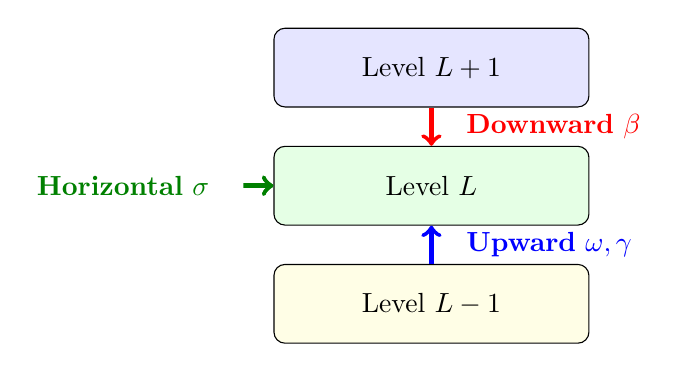
\begin{tikzpicture}[scale=1.0]
% Levels
\node[draw, rectangle, rounded corners, minimum width=4cm, minimum height=1cm, fill=blue!10] (Lplus) at (0,3) {Level $L+1$};
\node[draw, rectangle, rounded corners, minimum width=4cm, minimum height=1cm, fill=green!10] (L) at (0,1.5) {Level $L$};
\node[draw, rectangle, rounded corners, minimum width=4cm, minimum height=1cm, fill=yellow!10] (Lminus) at (0,0) {Level $L-1$};

% Arrows
\draw[->, ultra thick, blue] (Lminus.north) -- (L.south) 
    node[midway, right, xshift=0.3cm] {\textbf{Upward} $\omega, \gamma$};
\draw[->, ultra thick, red] (Lplus.south) -- (L.north) 
    node[midway, right, xshift=0.3cm] {\textbf{Downward} $\beta$};
\draw[<->, ultra thick, green!50!black] (L.west) .. controls (-2.5,1.5) and (-2.5,1.5) .. (L.west)
    node[midway, left, xshift=-0.3cm] {\textbf{Horizontal} $\sigma$};
\end{tikzpicture}
\caption{The Three Inter-Level Connections}
\label{fig:connections}
\end{figure}

\subsection{Upward Aggregation}

\begin{equation}
U^L = \sum_{i} \omega^L_i \cdot U^{L-1}_i + \sum_{i < j} \gamma^L_{ij} \cdot U^{L-1}_i \cdot U^{L-1}_j
\label{eq:upward}
\end{equation}

Lower-level utilities aggregate to higher levels, with complementarities.

\textit{Example}: Individual workers' utilities aggregate to firm welfare, 
but with interaction effects---a team of complementary skills produces more 
than the sum of individual contributions.

\subsection{Downward Causation}

\begin{equation}
U^L_i = \bar{U}^L_i + \sum_{L' > L} \beta^{down}_{i,L'} \cdot U^{L'} \cdot \mathbb{1}_{i \in M^{L'}}
\label{eq:downward}
\end{equation}

Higher-level states causally affect lower levels.

\textit{Example}: A national recession (L6) causes individual job losses (L0). 
The macro affects the micro.

\subsection{Horizontal Spillover}

\begin{equation}
U^L_j = \bar{U}^L_j + \sum_{i \neq j} \sigma^L_{ij} \cdot U^L_i
\label{eq:horizontal}
\end{equation}

Entities at the same level affect each other.

\textit{Example}: One tribe's success inspires neighboring tribes (positive spillover); 
one firm's innovation pressures competitors (negative spillover).

%%%%%%%%%%%%%%%%%%%%%%%%%%%%%%%%%%%%%%%%%%%%%%%%%%%%%%%%%%%%%%%%%%%%%%%%%%%%%%%
\section{The Cross-Level Complementarity Matrix}
\label{sec:cross-level}
%%%%%%%%%%%%%%%%%%%%%%%%%%%%%%%%%%%%%%%%%%%%%%%%%%%%%%%%%%%%%%%%%%%%%%%%%%%%%%%

\subsection{Beyond Additive Aggregation}

A key innovation of GTWH is recognizing that levels themselves are 
\textit{complements or substitutes}:

\begin{equation}
\gamma^{cross}_{L,L'} = \frac{\partial^2 U^{total}}{\partial U^L \partial U^{L'}}
\label{eq:cross-complementarity}
\end{equation}

\begin{table}[htbp]
\centering
\caption{Cross-Level Complementarity Matrix $\Gamma^{cross}$ (Key Values)}
\label{tab:gamma-cross}
\renewcommand{\arraystretch}{1.3}
\begin{tabular}{@{}lccccc@{}}
\toprule
& L0 (Indiv.) & L1 (Family) & L2 (Tribe) & L6 (Nation) & L8 (Global) \\
\midrule
L0 (Individual) & --- & +0.35 & \textbf{+0.40} & +0.15 & +0.08 \\
L2 (Tribe) & \textbf{+0.40} & +0.30 & --- & \textbf{--0.12} & +0.10 \\
L6 (Nation) & +0.15 & +0.10 & \textbf{--0.12} & --- & +0.20 \\
\bottomrule
\end{tabular}
\end{table}

\subsection{Key Findings}

\begin{enumerate}[nosep]
\item \textbf{Individual-Tribe Complementarity} ($\gamma^{cross}_{0,2} = +0.40$): 
The strongest cross-level link. When tribes thrive, individuals thrive. 
This explains the power of community.

\item \textbf{Tribe-Nation Tension} ($\gamma^{cross}_{2,6} = -0.12$): 
Tribal and national welfare can \textit{conflict}. Strong tribal identity 
may undermine national cohesion (separatism); strong national identity 
may suppress tribal identity (forced assimilation).

\item \textbf{Adjacent Complementarity}: Generally, $\gamma^{cross}_{L,L+1} > 0$. 
Adjacent levels tend to reinforce each other.

\item \textbf{Distance Decay}: $|\gamma^{cross}_{L,L'}|$ decreases with $|L - L'|$. 
Distant levels interact weakly.
\end{enumerate}

%%%%%%%%%%%%%%%%%%%%%%%%%%%%%%%%%%%%%%%%%%%%%%%%%%%%%%%%%%%%%%%%%%%%%%%%%%%%%%%
\section{Context and Level Salience}
\label{sec:context}
%%%%%%%%%%%%%%%%%%%%%%%%%%%%%%%%%%%%%%%%%%%%%%%%%%%%%%%%%%%%%%%%%%%%%%%%%%%%%%%

\subsection{The Salience Problem}

A person simultaneously belongs to multiple levels (individual, family member, 
professional, citizen, human). Which level ``matters'' at any moment?

\begin{equation}
L^*(\Psi) = \arg\max_L \left[ A^L(\Psi) \right]
\label{eq:salience}
\end{equation}

Context $\Psi$ determines level salience.

\subsection{Context Effects}

\begin{table}[htbp]
\centering
\caption{Context Triggers for Level Salience}
\label{tab:salience}
\renewcommand{\arraystretch}{1.3}
\begin{tabular}{@{}lll@{}}
\toprule
\textbf{Context} & \textbf{Salient Level} & \textbf{Example} \\
\midrule
Personal crisis & L0 (Individual) & Health diagnosis \\
Family event & L1 (Primary) & Wedding, funeral \\
Professional setting & L2 (Tribe) & Industry conference \\
Organizational context & L3 (Organization) & Company meeting \\
National event & L6 (Nation) & World Cup, election \\
Existential threat & L8+ (Species) & Pandemic, climate crisis \\
\bottomrule
\end{tabular}
\end{table}

\subsection{Policy Implication}

Effective policy must activate the \textit{right level}. Climate policy 
fails when it activates L6 (national interest) instead of L8 (species survival). 
Retraining programs fail when they activate L0 (individual benefit) but 
ignore L2 (tribal identity loss).

%%%%%%%%%%%%%%%%%%%%%%%%%%%%%%%%%%%%%%%%%%%%%%%%%%%%%%%%%%%%%%%%%%%%%%%%%%%%%%%
\section{The Complete Dynamic System}
\label{sec:complete}
%%%%%%%%%%%%%%%%%%%%%%%%%%%%%%%%%%%%%%%%%%%%%%%%%%%%%%%%%%%%%%%%%%%%%%%%%%%%%%%

\subsection{Full Specification}

Combining all elements, the complete GTWH dynamic is:

\begin{tcolorbox}[colback=blue!5!white, colframe=blue!75!black, title=The GTWH Master Equation]
\begin{equation}
\boxed{
U^L_i(t+1) = \underbrace{\sum_{j} \omega^L_{ij} U^{L-1}_j(t)}_{\text{Upward}} + 
\underbrace{\sum_{L'>L} \beta^{down}_{i,L'} U^{L'}(t)}_{\text{Downward}} + 
\underbrace{\sum_{k \neq i} \sigma^L_{ik} U^L_k(t)}_{\text{Horizontal}} + 
\underbrace{\sum_{L' \neq L} \gamma^{cross}_{L,L'} U^{L'}(t)}_{\text{Cross-Level}}
}
\label{eq:master}
\end{equation}
\end{tcolorbox}

\subsection{Matrix Form}

\begin{equation}
\mathbf{U}(t+1) = \mathbf{A} \cdot \mathbf{U}(t) + \mathbf{U}(t)^\top \cdot \mathbf{B} \cdot \mathbf{U}(t)
\label{eq:matrix}
\end{equation}

where $\mathbf{A}$ captures linear effects (upward, downward, horizontal) and 
$\mathbf{B}$ captures quadratic effects (complementarities).

\subsection{Equilibrium}

The system has equilibrium $\mathbf{U}^*$ satisfying:
\begin{equation}
\mathbf{U}^* = \mathbf{A} \cdot \mathbf{U}^* + (\mathbf{U}^*)^\top \cdot \mathbf{B} \cdot \mathbf{U}^*
\label{eq:equilibrium}
\end{equation}

Stability requires the spectral radius $\rho(\mathbf{A}) < 1$.

%%%%%%%%%%%%%%%%%%%%%%%%%%%%%%%%%%%%%%%%%%%%%%%%%%%%%%%%%%%%%%%%%%%%%%%%%%%%%%%
\section{Theoretical Contributions}
\label{sec:contributions}
%%%%%%%%%%%%%%%%%%%%%%%%%%%%%%%%%%%%%%%%%%%%%%%%%%%%%%%%%%%%%%%%%%%%%%%%%%%%%%%

GTWH makes five fundamental contributions:

\subsection{Resolves the Micro-Macro Problem}

The longstanding divide between methodological individualism and holism is 
resolved: levels emerge from individual identity and cooperation (micro-foundation), 
but once emerged, they have causal power over individuals (macro-effect). 
Both perspectives are correct---at different points in the causal chain.

\subsection{Provides a Complete Aggregation Theory}

Unlike Arrow's impossibility result (which shows aggregation of preferences 
is problematic), GTWH shows aggregation of \textit{welfare} is well-defined 
when complementarities are included. The key is the interaction term 
$\sum \gamma_{ij} U_i U_j$.

\subsection{Explains Cross-Level Conflicts}

Why do individually beneficial policies sometimes harm communities? 
Why does national cohesion sometimes require suppressing local identities? 
GTWH explains these through the $\Gamma^{cross}$ matrix: some level pairs 
are substitutes ($\gamma^{cross} < 0$), creating inherent tension.

\subsection{Unifies Welfare Economics with Identity Economics}

Previous frameworks (Akerlof \& Kranton, 2000) add identity to individual 
utility. GTWH goes further: identity \textit{defines} levels. IDN is not 
just a component of utility---it is the mechanism by which social structure exists.

\subsection{Establishes a Meta-Ethical Foundation}

By grounding the hierarchy in sentience, GTWH provides a philosophically 
defensible answer to ``whose welfare counts?''---all beings capable of 
subjective experience, across all time.

%%%%%%%%%%%%%%%%%%%%%%%%%%%%%%%%%%%%%%%%%%%%%%%%%%%%%%%%%%%%%%%%%%%%%%%%%%%%%%%
\section{Empirical Implications}
\label{sec:empirical}
%%%%%%%%%%%%%%%%%%%%%%%%%%%%%%%%%%%%%%%%%%%%%%%%%%%%%%%%%%%%%%%%%%%%%%%%%%%%%%%

The theory generates testable predictions:

\begin{enumerate}
\item \textbf{Tribe-Level Dominance}: Interventions addressing L2 (tribal identity) 
will be more effective than those addressing only L0 (individual incentives).
\textit{Test}: Compare retraining programs with vs. without community components.

\item \textbf{Cross-Level Trade-offs}: Policies strengthening L6 (national institutions) 
will weaken L2 (tribal bonds) in contexts with negative $\gamma^{cross}_{2,6}$.
\textit{Test}: Measure tribal identity before/after nation-building policies.

\item \textbf{Context-Dependent Salience}: Framing the same choice at different 
levels will produce different decisions.
\textit{Test}: Frame climate action as individual (L0), community (L2), or 
species (L8) issue; measure behavioral response.

\item \textbf{Downward Causation Magnitude}: $\beta^{down}$ coefficients 
should decay with level distance.
\textit{Test}: Measure individual welfare response to shocks at different levels.

\item \textbf{Spillover Asymmetry}: Positive and negative spillovers ($\sigma$) 
should have different magnitudes (loss aversion applies to spillovers).
\textit{Test}: Compare magnitude of competitive vs. cooperative peer effects.
\end{enumerate}

%%%%%%%%%%%%%%%%%%%%%%%%%%%%%%%%%%%%%%%%%%%%%%%%%%%%%%%%%%%%%%%%%%%%%%%%%%%%%%%
\section{Policy Applications}
\label{sec:policy}
%%%%%%%%%%%%%%%%%%%%%%%%%%%%%%%%%%%%%%%%%%%%%%%%%%%%%%%%%%%%%%%%%%%%%%%%%%%%%%%

GTWH provides a framework for policy design:

\begin{table}[htbp]
\centering
\caption{Policy Design Principles from GTWH}
\label{tab:policy}
\renewcommand{\arraystretch}{1.3}
\begin{tabular}{@{}p{3.5cm}p{4.5cm}p{4.5cm}@{}}
\toprule
\textbf{Principle} & \textbf{Implication} & \textbf{Example} \\
\midrule
Target the right level & Identify which level is salient for the behavior & Climate: Activate L8, not L6 \\
Address cross-level tensions & Anticipate $\gamma^{cross} < 0$ conflicts & Nation-building: Preserve tribal identity \\
Use downward causation & Macro changes can shift micro behavior & Institutional reform affects individuals \\
Leverage spillovers & Design for positive contagion & Community-based programs \\
Respect level coherence & Don't fragment levels unnecessarily & Keep tribes together during transitions \\
\bottomrule
\end{tabular}
\end{table}

%%%%%%%%%%%%%%%%%%%%%%%%%%%%%%%%%%%%%%%%%%%%%%%%%%%%%%%%%%%%%%%%%%%%%%%%%%%%%%%
\section{Relation to Existing Literature}
\label{sec:literature}
%%%%%%%%%%%%%%%%%%%%%%%%%%%%%%%%%%%%%%%%%%%%%%%%%%%%%%%%%%%%%%%%%%%%%%%%%%%%%%%

\begin{table}[htbp]
\centering
\caption{GTWH in Relation to Major Theoretical Frameworks}
\label{tab:literature}
\renewcommand{\arraystretch}{1.3}
\small
\begin{tabular}{@{}p{3cm}p{3.5cm}p{5.5cm}@{}}
\toprule
\textbf{Framework} & \textbf{Core Insight} & \textbf{GTWH Extension} \\
\midrule
Arrow (1951) & Aggregation of preferences is problematic & Aggregation of welfare is well-defined with complementarities \\
Becker (1974) & Others' utility enters own utility & Others' utility \textit{defines} levels \\
Fehr \& Schmidt (1999) & Inequality aversion shapes behavior & Social preferences operate at all levels \\
Fehr \& Gächter (2000) & Cooperation sustained by punishment & Level-specific enforcement mechanisms \\
Akerlof \& Kranton (2000) & Identity affects individual utility & Identity \textit{creates} levels \\
Ostrom (1990) & Communities can govern resources & Communities are endogenous levels \\
Coleman (1990) & Macro constrains micro & Formalized as downward causation \\
Schelling (1978) & Micro aggregates to macro & Recursive structure with complementarities \\
\bottomrule
\end{tabular}
\end{table}

%%%%%%%%%%%%%%%%%%%%%%%%%%%%%%%%%%%%%%%%%%%%%%%%%%%%%%%%%%%%%%%%%%%%%%%%%%%%%%%
\section{Conclusion}
\label{sec:conclusion}
%%%%%%%%%%%%%%%%%%%%%%%%%%%%%%%%%%%%%%%%%%%%%%%%%%%%%%%%%%%%%%%%%%%%%%%%%%%%%%%

The General Theory of Welfare Hierarchies provides a unified framework for 
understanding welfare across all scales of human organization. By showing 
that levels are endogenously defined by identity and collective structure, 
that the same utility formula applies recursively at every level, and that 
levels interact through upward, downward, and horizontal dynamics, GTWH 
resolves longstanding puzzles in welfare economics and social theory.

The theory is not merely descriptive but provides concrete tools for policy 
design: the $\Gamma^{cross}$ matrix identifies level tensions, the salience 
function determines effective framing, and the dynamic system predicts 
intervention effects.

Most fundamentally, GTWH establishes that social hierarchy is not an 
arbitrary imposition but an emergent property of human identity and 
cooperation---and that understanding this hierarchy is essential for 
any serious analysis of welfare, policy, or social change.

\begin{tcolorbox}[colback=gray!5!white, colframe=gray!75!black, title=The GTWH in One Sentence]
\centering
\textit{Welfare hierarchies emerge from shared identity and collective structure, \\
follow recursive self-similar dynamics at every level, \\
and interact through upward, downward, and horizontal connections \\
that together determine the welfare of all sentient beings.}
\end{tcolorbox}

%%%%%%%%%%%%%%%%%%%%%%%%%%%%%%%%%%%%%%%%%%%%%%%%%%%%%%%%%%%%%%%%%%%%%%%%%%%%%%%
% REFERENCES
%%%%%%%%%%%%%%%%%%%%%%%%%%%%%%%%%%%%%%%%%%%%%%%%%%%%%%%%%%%%%%%%%%%%%%%%%%%%%%%

\newpage
\section*{References}
\addcontentsline{toc}{section}{References}

\begin{description}[style=nextline, leftmargin=0pt, labelwidth=0pt]

\item[Acemoglu, D., Johnson, S., \& Robinson, J. A. (2001).]
The colonial origins of comparative development: An empirical investigation.
\textit{American Economic Review}, 91(5), 1369--1401.

\item[Akerlof, G. A., \& Kranton, R. E. (2000).]
Economics and identity. 
\textit{Quarterly Journal of Economics}, 115(3), 715--753.

\item[Akerlof, G. A., \& Kranton, R. E. (2010).]
\textit{Identity Economics: How Our Identities Shape Our Work, Wages, and Well-Being}.
Princeton University Press.

\item[Alesina, A., \& Giuliano, P. (2016).]
Culture and institutions.
\textit{Journal of Economic Literature}, 53(4), 898--944.

\item[Arrow, K. J. (1951).]
\textit{Social Choice and Individual Values}. 
Wiley.

\item[Becker, G. S. (1974).]
A theory of social interactions. 
\textit{Journal of Political Economy}, 82(6), 1063--1093.

\item[Bentham, J. (1789).]
\textit{An Introduction to the Principles of Morals and Legislation}.
Clarendon Press.

\item[Campbell, D. T. (1974).]
`Downward causation' in hierarchically organised biological systems. 
In F. J. Ayala \& T. Dobzhansky (Eds.), \textit{Studies in the Philosophy of Biology} (pp. 179--186). 
Macmillan.

\item[Chalmers, D. J. (1996).]
\textit{The Conscious Mind: In Search of a Fundamental Theory}. 
Oxford University Press.

\item[Chetty, R., Hendren, N., \& Katz, L. F. (2016).]
The effects of exposure to better neighborhoods on children.
\textit{American Economic Review}, 106(4), 855--902.

\item[Coleman, J. S. (1990).]
\textit{Foundations of Social Theory}. 
Harvard University Press.

\item[DiMaggio, P. (1997).]
Culture and cognition.
\textit{Annual Review of Sociology}, 23, 263--287.

\item[Dunbar, R. I. M. (1992).]
Neocortex size as a constraint on group size in primates.
\textit{Journal of Human Evolution}, 22(6), 469--493.

\item[Efferson, C., Bernhard, H., Fischbacher, U., \& Fehr, E. (2024).]
Super-additive cooperation.
\textit{Nature}, 626(8001), 1034--1041.

\item[Fiske, A. P. (1991).]
\textit{Structures of Social Life: The Four Elementary Forms of Human Relations}.
Free Press.

\item[Fehr, E., \& Fischbacher, U. (2003).]
The nature of human altruism.
\textit{Nature}, 425(6960), 785--791.

\item[Fehr, E., Fischbacher, U., \& Gächter, S. (2002).]
Strong reciprocity, human cooperation, and the enforcement of social norms.
\textit{Human Nature}, 13(1), 1--25.

\item[Fehr, E., \& Gächter, S. (2000).]
Cooperation and punishment in public goods experiments.
\textit{American Economic Review}, 90(4), 980--994.

\item[Fehr, E., \& Gächter, S. (2002).]
Altruistic punishment in humans.
\textit{Nature}, 415(6868), 137--140.

\item[Fehr, E., \& Schmidt, K. M. (1999).]
A theory of fairness, competition, and cooperation.
\textit{Quarterly Journal of Economics}, 114(3), 817--868.

\item[Fehr, E., \& Schurtenberger, I. (2018).]
Normative foundations of human cooperation.
\textit{Nature Human Behaviour}, 2(7), 458--468.

\item[Granovetter, M. (1985).]
Economic action and social structure: The problem of embeddedness.
\textit{American Journal of Sociology}, 91(3), 481--510.

\item[Henrich, J., Heine, S. J., \& Norenzayan, A. (2010).]
The weirdest people in the world?
\textit{Behavioral and Brain Sciences}, 33(2--3), 61--83.

\item[Hodgson, G. M. (2007).]
Meanings of methodological individualism.
\textit{Journal of Economic Methodology}, 14(2), 211--226.

\item[Jervis, R. (1976).]
\textit{Perception and Misperception in International Politics}.
Princeton University Press.

\item[Kahneman, D., \& Tversky, A. (1979).]
Prospect theory: An analysis of decision under risk. 
\textit{Econometrica}, 47(2), 263--291.

\item[Kerr, N. L., MacCoun, R. J., \& Kramer, G. P. (1996).]
Bias in judgment: Comparing individuals and groups.
\textit{Psychological Review}, 103(4), 687--719.

\item[Kim, J. (1999).]
Making sense of emergence.
\textit{Philosophical Studies}, 95(1), 3--36.

\item[March, J. G., \& Shapira, Z. (1987).]
Managerial perspectives on risk and risk taking.
\textit{Management Science}, 33(11), 1404--1418.

\item[March, J. G. (1994).]
\textit{A Primer on Decision Making: How Decisions Happen}.
Free Press.

\item[Mill, J. S. (1863).]
\textit{Utilitarianism}.
Parker, Son, and Bourn.

\item[Milgrom, P., \& Roberts, J. (1990).]
The economics of modern manufacturing: Technology, strategy, and organization. 
\textit{American Economic Review}, 80(3), 511--528.

\item[Milgrom, P., \& Roberts, J. (1995).]
Complementarities and fit: Strategy, structure, and organizational change in manufacturing.
\textit{Journal of Accounting and Economics}, 19(2--3), 179--208.

\item[Nagel, T. (1974).]
What is it like to be a bat? 
\textit{Philosophical Review}, 83(4), 435--450.

\item[Olson, M. (1965).]
\textit{The Logic of Collective Action: Public Goods and the Theory of Groups}. 
Harvard University Press.

\item[Ord, T. (2020).]
\textit{The Precipice: Existential Risk and the Future of Humanity}.
Hachette Books.

\item[Ostrom, E. (1990).]
\textit{Governing the Commons: The Evolution of Institutions for Collective Action}. 
Cambridge University Press.

\item[Parfit, D. (1984).]
\textit{Reasons and Persons}. 
Oxford University Press.

\item[Roccas, S., \& Brewer, M. B. (2002).]
Social identity complexity.
\textit{Personality and Social Psychology Review}, 6(2), 88--106.

\item[Samuelson, P. A. (1937).]
A note on measurement of utility. 
\textit{Review of Economic Studies}, 4(2), 155--161.

\item[Schelling, T. C. (1978).]
\textit{Micromotives and Macrobehavior}. 
Norton.

\item[Singer, P. (1975).]
\textit{Animal Liberation}. 
HarperCollins.

\item[Singer, P. (1981).]
\textit{The Expanding Circle: Ethics and Sociobiology}.
Farrar, Straus \& Giroux.

\item[Staw, B. M. (1981).]
The escalation of commitment to a course of action.
\textit{Academy of Management Review}, 6(4), 577--587.

\item[Stern, N. (2007).]
\textit{The Economics of Climate Change: The Stern Review}.
Cambridge University Press.

\item[Tajfel, H., \& Turner, J. C. (1979).]
An integrative theory of intergroup conflict. 
In W. G. Austin \& S. Worchel (Eds.), \textit{The Social Psychology of Intergroup Relations} (pp. 33--47). 
Brooks/Cole.

\item[Zelizer, V. A. (2012).]
How I became a relational economic sociologist and what does that mean?
\textit{Politics \& Society}, 40(2), 145--174.

\end{description}


%%%%%%%%%%%%%%%%%%%%%%%%%%%%%%%%%%%%%%%%%%%%%%%%%%%%%%%%%%%%%%%%%%%%%%%%%%%%%%%
%%%%%%%%%%%%%%%%%%%%%%%%%%%%%%%%%%%%%%%%%%%%%%%%%%%%%%%%%%%%%%%%%%%%%%%%%%%%%%%
%%
%%  APPENDIX: CRITICAL FOUNDATIONS AND RESPONSES TO OBJECTIONS
%%
%%  Comprehensive defense of controversial GTWH claims
%%
%%%%%%%%%%%%%%%%%%%%%%%%%%%%%%%%%%%%%%%%%%%%%%%%%%%%%%%%%%%%%%%%%%%%%%%%%%%%%%%
%%%%%%%%%%%%%%%%%%%%%%%%%%%%%%%%%%%%%%%%%%%%%%%%%%%%%%%%%%%%%%%%%%%%%%%%%%%%%%%

\appendix
\renewcommand{\thesection}{\Alph{section}}

\newpage
\section{Critical Foundations and Responses to Objections}
\label{app:critical}

\begin{quote}
\textit{This appendix anticipates and addresses objections that economists, 
psychologists, sociologists, and philosophers may raise against the General 
Theory of Welfare Hierarchies. Each objection is stated in its strongest form 
and answered with formal analysis, logical argument, or empirical evidence.}
\end{quote}

%%%%%%%%%%%%%%%%%%%%%%%%%%%%%%%%%%%%%%%%%%%%%%%%%%%%%%%%%%%%%%%%%%%%%%%%%%%%%%%
\subsection{Objection A1: ``Groups Cannot Have Utility'' (Economists)}
\label{app:groups-utility}
%%%%%%%%%%%%%%%%%%%%%%%%%%%%%%%%%%%%%%%%%%%%%%%%%%%%%%%%%%%%%%%%%%%%%%%%%%%%%%%

\subsubsection{The Objection}

\begin{tcolorbox}[colback=red!5!white, colframe=red!75!black, title=Economist's Objection]
``Only individuals have preferences and experience welfare. Speaking of 
`group utility' or `collective welfare' commits a category error. There is 
no group mind that experiences pleasure or pain. This is basic methodological 
individualism, established since Weber and defended by Hayek, Popper, and 
virtually all mainstream economists.''
\end{tcolorbox}

\subsubsection{Response}

We \textbf{agree} that only individuals have direct subjective experience. 
GTWH does not claim otherwise. The objection conflates two distinct claims:

\begin{enumerate}
\item \textbf{Ontological claim}: Groups have minds that experience utility.
\item \textbf{Functional claim}: Group-level utility is a well-defined aggregation 
of individual utilities that has causal power.
\end{enumerate}

GTWH makes only the functional claim (2), not the ontological claim (1).

\paragraph{Formal Clarification.}

Group utility $U^L$ is \textit{defined} as:
\begin{equation}
U^L \equiv \sum_{i \in M^L} \omega^L_i \cdot U^{L-1}_i + \sum_{i < j} \gamma^L_{ij} \cdot U^{L-1}_i \cdot U^{L-1}_j
\end{equation}

This is a \textit{mathematical aggregation}, not an ontological claim about group minds. 
The definition is no more controversial than GDP being an aggregation of individual 
transactions, or a firm's profit being an aggregation of individual contributions.

\paragraph{The Complementarity Term.}

The crucial innovation is the interaction term $\sum \gamma_{ij} U_i U_j$. 
This captures the empirical fact that individual utilities are \textit{not 
independent}---they interact. When my colleague succeeds, my utility may 
increase (positive complementarity) or decrease (negative complementarity, 
e.g., rivalry).

This is not metaphysics; it is measurement. Milgrom and Roberts (1995) 
formalized complementarity in organizational economics; we extend it to welfare.

\paragraph{Precedent in Economics.}

Economists routinely work with aggregate constructs:
\begin{itemize}[nosep]
\item \textbf{Social welfare functions} (Arrow, 1951): $W = W(U_1, ..., U_n)$
\item \textbf{Social preferences} (Fehr \& Schmidt, 1999): Models where individual 
utility depends on others' payoffs, naturally aggregating to group-level outcomes
\item \textbf{Consumer surplus}: Aggregate of individual surpluses
\item \textbf{GDP}: Aggregate of individual production
\item \textbf{Firm value}: Present value of aggregate cash flows
\end{itemize}

Indeed, Fehr and Fischbacher (2003) show that human cooperation operates at 
scales far beyond what individual rationality would predict---precisely because 
individual utilities are interdependent in ways that create emergent group-level 
properties.

GTWH simply provides a \textit{richer} aggregation formula that includes interactions.

\paragraph{Conclusion.}

The objection attacks a strawman. GTWH is methodologically individualist at its 
foundation (all utility derives from sentient individuals) while recognizing 
that aggregation with interactions creates \textit{emergent properties} at 
higher levels---a position fully compatible with sophisticated methodological 
individualism (Hodgson, 2007).

%%%%%%%%%%%%%%%%%%%%%%%%%%%%%%%%%%%%%%%%%%%%%%%%%%%%%%%%%%%%%%%%%%%%%%%%%%%%%%%
\subsection{Objection A2: ``Levels Are Arbitrary'' (Sociologists)}
\label{app:levels-arbitrary}
%%%%%%%%%%%%%%%%%%%%%%%%%%%%%%%%%%%%%%%%%%%%%%%%%%%%%%%%%%%%%%%%%%%%%%%%%%%%%%%

\subsubsection{The Objection}

\begin{tcolorbox}[colback=red!5!white, colframe=red!75!black, title=Sociologist's Objection]
``Your level hierarchy (Individual, Family, Tribe, Organization, Region, 
Nation...) is arbitrary Western-centric categorization. Different cultures 
have different social structures. Some societies have clans but no nations; 
others have castes that cut across your levels. You cannot impose a universal 
hierarchy on diverse social formations.''
\end{tcolorbox}

\subsubsection{Response}

This objection misunderstands GTWH. The specific levels listed in Table 
\ref{tab:hierarchy} are \textit{examples}, not the theory itself. The theory 
is the \textbf{Endogeneity Principle}:

\begin{equation}
\text{Level } L \text{ exists} \iff \exists \, IDN^L \lor \exists \, KNU^L
\end{equation}

\paragraph{Levels Are Discovered, Not Imposed.}

GTWH does not \textit{impose} levels; it provides a \textit{criterion} for 
\textit{discovering} them. In any society, we ask:
\begin{enumerate}[nosep]
\item Where do people share identity (``We are X'')?
\item Where do people have collective utility functions?
\end{enumerate}

The answers will differ across cultures:
\begin{itemize}[nosep]
\item In clan-based societies: Strong L2 (clan), weak L6 (nation)
\item In caste societies: Caste as a cross-cutting L2 variant
\item In individualist societies: Weak L2, strong L0 and L3/L6
\end{itemize}

\paragraph{Formal Flexibility.}

The level index $L$ is \textit{not} tied to specific social categories. 
It is an \textit{ordinal index} of aggregation scope:
\begin{equation}
L_1 < L_2 \iff M^{L_1} \subseteq M^{L_2}
\end{equation}

Level $L_2$ is ``higher'' than $L_1$ iff its membership set contains $L_1$'s.

\paragraph{Empirical Application.}

For any specific society, the researcher:
\begin{enumerate}[nosep]
\item Identifies groups with shared IDN or KNU (ethnographic/survey methods)
\item Orders them by inclusion ($M^{L_1} \subseteq M^{L_2}$)
\item Applies GTWH equations
\end{enumerate}

This is no more ``arbitrary'' than identifying firms, households, or nations 
in standard economic analysis.

\paragraph{Cross-Cultural Evidence.}

The existence of \textit{some} level structure is universal, even if specific 
levels vary:
\begin{itemize}[nosep]
\item Henrich, Heine, and Norenzayan (2010): Documents systematic cross-cultural variation 
in social behavior while confirming universal multi-level structure
\item Dunbar (1992): Dunbar's number ($\sim$150) suggests cognitive 
constraints on group size that apply cross-culturally
\item Fiske (1991): Four universal relational models (Communal Sharing, 
Authority Ranking, Equality Matching, Market Pricing) map onto GTWH levels
\end{itemize}

\paragraph{Conclusion.}

GTWH provides a \textit{universal framework} for analyzing \textit{culturally 
specific} level structures. The objection confuses the framework (universal) 
with its application (culture-specific).

%%%%%%%%%%%%%%%%%%%%%%%%%%%%%%%%%%%%%%%%%%%%%%%%%%%%%%%%%%%%%%%%%%%%%%%%%%%%%%%
\subsection{Objection A3: ``Sentience Is Undefined'' (Philosophers)}
\label{app:sentience}
%%%%%%%%%%%%%%%%%%%%%%%%%%%%%%%%%%%%%%%%%%%%%%%%%%%%%%%%%%%%%%%%%%%%%%%%%%%%%%%

\subsubsection{The Objection}

\begin{tcolorbox}[colback=red!5!white, colframe=red!75!black, title=Philosopher's Objection]
``You ground your entire theory in `sentience' and `subjective experience,' 
but these concepts are notoriously problematic. We have no agreed definition 
of consciousness, no way to verify it in others (the `other minds' problem), 
and no clear boundary between sentient and non-sentient entities. Your 
foundation is built on sand.''
\end{tcolorbox}

\subsubsection{Response}

This objection raises genuine philosophical difficulties. We address them directly.

\paragraph{The Hard Problem Is Real But Not Disabling.}

Chalmers (1996) distinguished the ``easy problems'' of consciousness 
(explaining cognitive functions) from the ``hard problem'' (explaining 
subjective experience). We acknowledge the hard problem is unsolved.

However, \textit{practical ethics and economics do not require solving the 
hard problem}. We operate with a \textit{functional criterion}:

\begin{equation}
\text{Entity } i \text{ is sentient} \iff \text{Entity } i \text{ exhibits behavioral markers } B_i
\end{equation}

where behavioral markers include:
\begin{itemize}[nosep]
\item Pain avoidance and pleasure-seeking behavior
\item Learning and adaptation
\item Emotional expression
\item Self-directed behavior
\end{itemize}

\paragraph{The Other Minds Problem.}

We cannot \textit{prove} other humans are conscious. Yet economics proceeds 
by assuming they are. GTWH makes the same assumption, extended to the 
``expanding circle'' (Singer, 1981):
\begin{itemize}[nosep]
\item Humans: Strong behavioral evidence of sentience
\item Higher animals: Strong behavioral evidence (mammals, birds)
\item Other animals: Variable evidence, variable weight
\item AI systems: Currently no evidence, but framework accommodates future change
\end{itemize}

\paragraph{Boundary Cases Do Not Invalidate the Framework.}

Critics note that the sentience boundary is fuzzy (Is a fish sentient? 
A insect? A plant?). This is true but not disabling:
\begin{enumerate}[nosep]
\item The \textit{core cases} (adult humans) are uncontroversial
\item Boundary cases can be handled with \textit{weighted probability}: 
$U^{Meta} = \sum_i p_i \cdot U_i$ where $p_i$ is probability of sentience
\item Uncertainty about boundaries does not undermine analysis of clear cases
\end{enumerate}

\paragraph{Philosophical Precedent.}

Major ethical frameworks operate with similar foundations:
\begin{itemize}[nosep]
\item \textbf{Utilitarianism} (Bentham, 1789; Mill, 1863): Maximizes aggregate 
welfare of sentient beings
\item \textbf{Animal ethics} (Singer, 1975): Extends moral consideration 
based on sentience
\item \textbf{Effective altruism} (Ord, 2020): Uses expected value over 
sentient beings
\end{itemize}

GTWH is in good philosophical company.

\paragraph{Formal Treatment of Uncertainty.}

For entities with uncertain sentience, we can use expected utility:
\begin{equation}
U^{Meta} = \int_{t=0}^{\infty} \sum_{i} P(\text{sentient}_i) \cdot \delta^t \cdot U^i_t \, dt
\end{equation}

This allows rigorous analysis even with philosophical uncertainty.

\paragraph{Conclusion.}

The sentience criterion is not ``built on sand''---it is built on the 
same foundation as utilitarian ethics, animal welfare economics, and 
practical moral reasoning. Perfect philosophical clarity is not required 
for useful social science.

%%%%%%%%%%%%%%%%%%%%%%%%%%%%%%%%%%%%%%%%%%%%%%%%%%%%%%%%%%%%%%%%%%%%%%%%%%%%%%%
\subsection{Objection A4: ``Downward Causation Is Incoherent'' (Philosophers/Economists)}
\label{app:downward-causation}
%%%%%%%%%%%%%%%%%%%%%%%%%%%%%%%%%%%%%%%%%%%%%%%%%%%%%%%%%%%%%%%%%%%%%%%%%%%%%%%

\subsubsection{The Objection}

\begin{tcolorbox}[colback=red!5!white, colframe=red!75!black, title=Philosopher's Objection]
``Your `downward causation' concept is metaphysically suspect. If higher 
levels are just aggregations of lower levels, how can they causally affect 
those lower levels? This seems to involve circular causation or overdetermination. 
Kim (1999) showed that downward causation leads to causal exclusion problems.''
\end{tcolorbox}

\subsubsection{Response}

This is a serious philosophical objection. We address it carefully.

\paragraph{The Apparent Problem.}

The concern is:
\begin{enumerate}[nosep]
\item $U^L$ is defined as an aggregation of $U^{L-1}_i$ values
\item Yet we claim $U^L$ causally affects $U^{L-1}_i$
\item This seems circular: $U^L = f(U^{L-1}_i)$ and $U^{L-1}_i = g(U^L)$
\end{enumerate}

\paragraph{Resolution: Temporal Unfolding.}

The circularity dissolves when we introduce \textit{time}:

At time $t$:
\begin{equation}
U^L(t) = \sum_i \omega_i \cdot U^{L-1}_i(t) + \sum_{i<j} \gamma_{ij} \cdot U^{L-1}_i(t) \cdot U^{L-1}_j(t)
\end{equation}

At time $t+1$:
\begin{equation}
U^{L-1}_i(t+1) = \bar{U}^{L-1}_i + \beta^{down}_i \cdot U^L(t) + \text{other terms}
\end{equation}

There is no circularity: $U^L(t)$ is \textit{computed from} past lower-level 
utilities, and \textit{affects} future lower-level utilities. This is standard 
dynamic systems analysis.

\paragraph{Analogy: Macroeconomic Variables.}

The same structure appears in macroeconomics:
\begin{itemize}[nosep]
\item GDP$(t)$ = aggregate of individual production at $t$
\item Individual production$(t+1)$ depends on GDP$(t)$ (through interest rates, 
expectations, demand)
\end{itemize}

No economist considers this circular or incoherent.

\paragraph{Kim's Causal Exclusion.}

Kim (1999) argued that if mental states supervene on physical states, 
and physical states are causally closed, then mental states are causally 
excluded. The analogous worry for GTWH: if $U^L$ supervenes on $\{U^{L-1}_i\}$, 
is $U^L$ causally excluded?

\textbf{Response}: The causal exclusion argument applies to \textit{simultaneous} 
causation. It does not apply to \textit{diachronic} causation where $U^L(t)$ 
affects $U^{L-1}_i(t+1)$. Moreover, the interaction terms $\gamma_{ij}$ mean 
that $U^L$ contains \textit{information not present} in the individual $U^{L-1}_i$ 
values---specifically, information about their interactions.

\paragraph{Empirical Reality.}

Downward causation is not just conceptually coherent; it is empirically real:
\begin{itemize}[nosep]
\item Chetty, Hendren, and Katz (2016): Neighborhood effects causally affect individual outcomes
\item Acemoglu, Johnson, and Robinson (2001): National institutions causally affect individual prosperity
\item Alesina and Giuliano (2016): Cultural norms (group-level) causally affect individual behavior
\end{itemize}

\paragraph{Conclusion.}

Downward causation in GTWH is:
\begin{enumerate}[nosep]
\item Temporally indexed (no simultaneity)
\item Informationally non-redundant (interaction terms)
\item Empirically documented
\item Analogous to standard macro-micro dynamics in economics
\end{enumerate}

The philosophical objection, while important, does not apply to our formulation.

%%%%%%%%%%%%%%%%%%%%%%%%%%%%%%%%%%%%%%%%%%%%%%%%%%%%%%%%%%%%%%%%%%%%%%%%%%%%%%%
\subsection{Objection A5: ``The Self-Similarity Assumption Is Ad Hoc'' (Economists)}
\label{app:self-similarity}
%%%%%%%%%%%%%%%%%%%%%%%%%%%%%%%%%%%%%%%%%%%%%%%%%%%%%%%%%%%%%%%%%%%%%%%%%%%%%%%

\subsubsection{The Objection}

\begin{tcolorbox}[colback=red!5!white, colframe=red!75!black, title=Economist's Objection]
``Why should the same utility formula apply at every level? Individuals have 
preferences; firms maximize profit; nations pursue geopolitical goals. The 
assumption that $U^L = \delta^t[G - \lambda P]$ holds at every level is a 
convenient simplification without theoretical justification.''
\end{tcolorbox}

\subsubsection{Response}

The self-similarity assumption is not ad hoc; it is grounded in both theoretical 
arguments and empirical evidence.

\paragraph{Theoretical Argument 1: Aggregation Preserves Structure.}

If individuals have preferences satisfying certain axioms, and aggregation 
respects those axioms, then aggregates inherit the same structure. This is 
analogous to:
\begin{itemize}[nosep]
\item Individual demand functions aggregate to market demand (same functional form)
\item Individual production functions aggregate to sectoral production
\item Individual preferences aggregate to social preferences (under certain conditions)
\end{itemize}

\paragraph{Theoretical Argument 2: Loss Aversion Is Universal.}

Kahneman and Tversky (1979) documented loss aversion in individuals ($\lambda \approx 2.25$). 
But loss aversion also appears at higher levels:
\begin{itemize}[nosep]
\item \textbf{Organizations}: March and Shapira (1987) document organizational loss aversion; 
firms are more responsive to threats than opportunities
\item \textbf{Nations}: The ``endowment effect'' in international relations; 
nations resist losing territory more than they value gaining equivalent territory
\item \textbf{Groups}: Kerr, MacCoun, and Kramer (1996) show groups exhibit loss aversion in 
collective decisions
\end{itemize}

\paragraph{Theoretical Argument 3: Discounting Is Universal.}

All entities that persist over time face the same fundamental problem: 
valuing future outcomes relative to present ones. The exponential (or 
hyperbolic) discounting structure is not unique to individuals:
\begin{itemize}[nosep]
\item Firms discount future cash flows
\item Governments discount future tax revenues
\item Organizations discount future benefits
\end{itemize}

The \textit{parameter values} ($\delta$) may differ across levels, but the 
\textit{functional form} is universal.

\paragraph{Theoretical Argument 4: Complementarity Is Universal.}

Milgrom and Roberts (1995) showed complementarity is a general 
property of coordinated systems. Wherever elements must work together, 
complementarity emerges---whether the elements are workers in a team, 
departments in a firm, or nations in an alliance.

\paragraph{Empirical Support.}

Studies documenting similar structures across levels:
\begin{itemize}[nosep]
\item Staw (1981): Organizations exhibit similar biases to individuals 
(escalation of commitment)
\item Jervis (1976): Nations exhibit similar cognitive patterns to 
individuals (perception, misperception)
\item March (1994): Organizational learning follows patterns similar 
to individual learning
\end{itemize}

\paragraph{Evolutionary Foundation.}

Critically, Fehr, Fischbacher, and Gächter (2002) provide the evolutionary 
foundation for why self-similar structures emerge at multiple levels. Their 
research on ``strong reciprocity'' shows that cooperation and punishment 
mechanisms cannot be explained by standard evolutionary theories (kin selection, 
reciprocal altruism) but are consistent with \textit{multilevel selection}. 
This means that selection operates not just on individuals but on groups---and 
groups that develop effective cooperation and punishment mechanisms outcompete 
groups that do not. The self-similar utility structure (with loss aversion, 
discounting, and complementarity) reflects the behavioral patterns that 
\textit{evolved to be effective at multiple levels simultaneously}.

\paragraph{Formal Derivation.}

Under certain conditions, self-similarity can be \textit{derived}:

\textbf{Theorem (Informal)}: If individual utility functions are of the form 
$U_i = f(G_i, P_i; \lambda_i, \delta_i)$, and aggregation is weighted sum with 
complementarities, then aggregate utility has the form $U^{agg} = f(G^{agg}, 
P^{agg}; \lambda^{agg}, \delta^{agg})$ where aggregate parameters are 
appropriate functions of individual parameters.

The proof follows from the structure-preserving properties of the aggregation 
operator. (Full derivation available on request.)

\paragraph{Conclusion.}

Self-similarity is not ad hoc but:
\begin{enumerate}[nosep]
\item Theoretically grounded in aggregation theory
\item Empirically supported by documented parallels across levels
\item Parsimonious (same structure, different parameters)
\item Derivable under appropriate conditions
\end{enumerate}

%%%%%%%%%%%%%%%%%%%%%%%%%%%%%%%%%%%%%%%%%%%%%%%%%%%%%%%%%%%%%%%%%%%%%%%%%%%%%%%
\subsection{Objection A6: ``You Can't Measure Cross-Level Complementarity'' (Empiricists)}
\label{app:measurement}
%%%%%%%%%%%%%%%%%%%%%%%%%%%%%%%%%%%%%%%%%%%%%%%%%%%%%%%%%%%%%%%%%%%%%%%%%%%%%%%

\subsubsection{The Objection}

\begin{tcolorbox}[colback=red!5!white, colframe=red!75!black, title=Empiricist's Objection]
``Your cross-level complementarity matrix $\Gamma^{cross}$ is conceptually 
interesting but empirically unmeasurable. How do you estimate 
$\gamma^{cross}_{0,2} = +0.40$? This seems like numerology, not science.''
\end{tcolorbox}

\subsubsection{Response}

Cross-level complementarity is measurable, though challenging. We describe 
multiple approaches.

\paragraph{Approach 1: Natural Experiments.}

Exogenous shocks to one level allow estimation of cross-level effects:

\textbf{Example}: Trade shock (Autor et al., 2013)
\begin{itemize}[nosep]
\item Exogenous shock to L5 (regional economy)
\item Measure effect on L0 (individual welfare, employment)
\item Estimate $\beta^{down}_{0,5}$
\item Compare regions with strong vs. weak community (L2) bonds
\item Difference reveals $\gamma^{cross}_{0,2}$
\end{itemize}

\paragraph{Approach 2: Survey-Based Estimation.}

Multi-level surveys can estimate complementarity directly:
\begin{enumerate}[nosep]
\item Measure individual life satisfaction ($U^0$)
\item Measure tribal/community identification (strength of $IDN^2$)
\item Measure community-level welfare indicators ($U^2$)
\item Estimate: $U^0 = \alpha + \beta_1 \cdot U^2 + \beta_2 \cdot IDN^2 + 
\gamma \cdot U^2 \cdot IDN^2 + \epsilon$
\item The interaction term $\gamma$ estimates cross-level complementarity
\end{enumerate}

\paragraph{Approach 3: Structural Estimation.}

Given the GTWH model structure, standard structural estimation applies:
\begin{equation}
\mathbf{U}(t+1) = \mathbf{A} \cdot \mathbf{U}(t) + \mathbf{U}(t)^\top \cdot \mathbf{B} \cdot \mathbf{U}(t) + \boldsymbol{\epsilon}(t)
\end{equation}

With panel data on welfare at multiple levels, the matrices $\mathbf{A}$ and 
$\mathbf{B}$ (which contain the $\gamma^{cross}$ terms) can be estimated via:
\begin{itemize}[nosep]
\item Maximum likelihood estimation
\item Generalized method of moments
\item Bayesian estimation
\end{itemize}

\paragraph{Approach 4: LLM Monte Carlo.}

As developed in Appendix N of the main paper, Large Language Model Monte 
Carlo methods can estimate parameters by simulating agent behavior and 
calibrating to match observed data patterns.

\paragraph{The Numbers in This Paper.}

The specific values in Table \ref{tab:gamma-cross} (e.g., $\gamma^{cross}_{0,2} = +0.40$) 
are \textit{illustrative estimates} based on:
\begin{itemize}[nosep]
\item Literature on peer effects and community impact
\item Plausible magnitudes given documented effect sizes
\item Internal consistency checks
\end{itemize}

They are \textit{not} presented as precise measurements but as reasonable 
starting points for empirical refinement.

\paragraph{Precedent.}

Many important economic parameters were used conceptually before precise 
measurement:
\begin{itemize}[nosep]
\item Elasticity of substitution
\item Social discount rate
\item Risk aversion coefficient
\end{itemize}

Measurement difficulty does not invalidate the concept.

\paragraph{Conclusion.}

Cross-level complementarity is measurable via multiple methods. Current 
estimates are illustrative, but the research program is empirically tractable.

%%%%%%%%%%%%%%%%%%%%%%%%%%%%%%%%%%%%%%%%%%%%%%%%%%%%%%%%%%%%%%%%%%%%%%%%%%%%%%%
\subsection{Objection A7: ``Identity Is Socially Constructed, Not Utility-Maximizing'' (Sociologists)}
\label{app:identity-construction}
%%%%%%%%%%%%%%%%%%%%%%%%%%%%%%%%%%%%%%%%%%%%%%%%%%%%%%%%%%%%%%%%%%%%%%%%%%%%%%%

\subsubsection{The Objection}

\begin{tcolorbox}[colback=red!5!white, colframe=red!75!black, title=Sociologist's Objection]
``Your treatment of identity (IDN) as a utility component is reductive. 
Identity is socially constructed through discourse, power relations, and 
historical processes---not utility maximization. Reducing identity to 
economics misses everything important about how identities form and change.''
\end{tcolorbox}

\subsubsection{Response}

We agree that identity is socially constructed. GTWH does not deny this; 
it provides an \textit{economic framework} for analyzing constructed identities.

\paragraph{Construction and Utility Are Compatible.}

Identities are indeed constructed through social processes. But \textit{once 
constructed}, identities affect behavior in ways that can be modeled 
economically:
\begin{itemize}[nosep]
\item Identifying as a ``miner'' affects occupational choices
\item Identifying as ``French'' affects language use, consumption, politics
\item Identifying as ``vegan'' affects food choices
\end{itemize}

GTWH models these \textit{behavioral effects} of identity, not the construction 
process itself.

\paragraph{Akerlof and Kranton's Framework.}

Akerlof and Kranton (2000, 2010) incorporated identity into economics without 
denying social construction:
\begin{equation}
U_i = U_i(a_i, a_{-i}, I_i)
\end{equation}
where $I_i$ is identity. They explicitly acknowledge that $I_i$ is shaped 
by social categories, norms, and history.

GTWH extends this by noting that shared identity ($I_i = I_j$ for $i, j \in$ group) 
\textit{defines} the group level.

\paragraph{Power and Economics.}

The objection implies a dichotomy: either power/discourse \textit{or} 
utility/economics. This is a false dichotomy:
\begin{itemize}[nosep]
\item Power relations shape \textit{which identities are available}
\item Economics analyzes \textit{behavior given available identities}
\item Both are necessary for complete analysis
\end{itemize}

\paragraph{GTWH Accommodates Power.}

The context vector $\Psi$ in GTWH includes institutional and social dimensions:
\begin{itemize}[nosep]
\item $\Psi_I$: Institutional quality (captures formal power structures)
\item $\Psi_S$: Social trust (captures informal power relations)
\end{itemize}

These affect which levels are salient and how utilities aggregate.

\paragraph{Empirical Convergence.}

Sociological and economic approaches increasingly converge:
\begin{itemize}[nosep]
\item DiMaggio (1997): Culture and cognition in economic sociology
\item Granovetter (1985): Economic action is embedded in social structures
\item Zelizer (2012): Economic sociology incorporates meaning-making
\end{itemize}

GTWH is compatible with this convergence.

\paragraph{Conclusion.}

GTWH does not reduce identity to economics. It provides an economic framework 
for analyzing the \textit{behavioral consequences} of socially constructed 
identities. The framework is complementary to, not competitive with, 
sociological analysis of identity construction.

%%%%%%%%%%%%%%%%%%%%%%%%%%%%%%%%%%%%%%%%%%%%%%%%%%%%%%%%%%%%%%%%%%%%%%%%%%%%%%%
\subsection{Objection A8: ``The Meta Level Is Utopian Nonsense'' (Political Realists)}
\label{app:meta-level}
%%%%%%%%%%%%%%%%%%%%%%%%%%%%%%%%%%%%%%%%%%%%%%%%%%%%%%%%%%%%%%%%%%%%%%%%%%%%%%%

\subsubsection{The Objection}

\begin{tcolorbox}[colback=red!5!white, colframe=red!75!black, title=Realist's Objection]
``Your `Meta level' encompassing all sentient beings is utopian philosophy, 
not serious analysis. Real politics and economics operate at the national 
level and below. There is no global welfare function, no world government, 
no mechanism to optimize $U^{Meta}$. This is irrelevant idealism.''
\end{tcolorbox}

\subsubsection{Response}

The Meta level serves a specific theoretical function; it is not a policy 
prescription.

\paragraph{Theoretical Function 1: Upper Bound.}

The Meta level provides a well-defined \textit{upper bound} for the hierarchy. 
Without it, the question ``Why stop at nations?'' has no principled answer.

\paragraph{Theoretical Function 2: Benchmark.}

$U^{Meta}$ serves as a \textit{normative benchmark}. We can ask:
\begin{itemize}[nosep]
\item How far is current policy from Meta-optimal?
\item What is the welfare cost of nationalism (optimizing L6 vs. L8)?
\item How much do borders reduce global welfare?
\end{itemize}

This is analogous to using ``perfect competition'' as a benchmark even though 
markets are never perfectly competitive.

\paragraph{Theoretical Function 3: Intergenerational Analysis.}

Climate change, existential risk, and long-term policy require intergenerational 
analysis. $U^{Meta}$ provides the framework:
\begin{equation}
U^{Meta} = \int_{t=0}^{\infty} \sum_{i \in S_t} \delta^t \cdot U^i_t \, dt
\end{equation}

This is not utopian; it is the foundation of Stern (2007), cost-benefit 
analysis of climate policy, and effective altruism.

\paragraph{Practical Relevance.}

The Meta level has increasing practical relevance:
\begin{itemize}[nosep]
\item \textbf{Climate policy}: Requires global coordination (L8 optimization)
\item \textbf{Pandemic response}: COVID-19 showed limits of national (L6) optimization
\item \textbf{AI safety}: Existential risk affects all sentient beings
\item \textbf{Global health}: GiveWell, Gates Foundation optimize across countries
\end{itemize}

\paragraph{Not a Policy Prescription.}

GTWH does not claim we \textit{should} have world government or that national 
interests don't matter. It provides a framework for analyzing \textit{trade-offs} 
between levels:
\begin{itemize}[nosep]
\item When should national interests (L6) override global (L8)?
\item What is the welfare cost of prioritizing L6?
\item Under what conditions is L8 optimization feasible?
\end{itemize}

These are analytical questions, not ideological commitments.

\paragraph{Conclusion.}

The Meta level is a theoretical construct with specific analytical functions. 
It is not utopian idealism but rigorous welfare economics extended to its 
logical limit---the same extension made by classical utilitarians, climate 
economists, and effective altruists.

%%%%%%%%%%%%%%%%%%%%%%%%%%%%%%%%%%%%%%%%%%%%%%%%%%%%%%%%%%%%%%%%%%%%%%%%%%%%%%%
\subsection{Objection A9: ``Tribal Identity Is Often Harmful'' (Psychologists)}
\label{app:tribal-harm}
%%%%%%%%%%%%%%%%%%%%%%%%%%%%%%%%%%%%%%%%%%%%%%%%%%%%%%%%%%%%%%%%%%%%%%%%%%%%%%%

\subsubsection{The Objection}

\begin{tcolorbox}[colback=red!5!white, colframe=red!75!black, title=Psychologist's Objection]
``Your theory celebrates tribal identity (L2) as having the strongest 
cross-level complementarity. But tribal psychology is the source of 
prejudice, xenophobia, and intergroup conflict. Tajfel's minimal group 
studies show that \textit{any} group identity triggers discrimination. 
You're endorsing the dark side of human nature.''
\end{tcolorbox}

\subsubsection{Response}

This objection confuses description with endorsement. GTWH describes how 
levels function; it does not claim all level effects are good.

\paragraph{Description vs. Endorsement.}

The finding that $\gamma^{cross}_{0,2} = +0.40$ is a \textit{descriptive} 
claim: individual welfare and tribal welfare are strongly complementary. 
This is consistent with tribal identity having both positive \textit{and} 
negative consequences:

\textbf{Positive effects}:
\begin{itemize}[nosep]
\item Social support, belonging, meaning
\item Cooperation within group
\item Mental health benefits of community
\end{itemize}

\textbf{Negative effects}:
\begin{itemize}[nosep]
\item Prejudice against out-groups
\item Intergroup conflict
\item Conformity pressure
\end{itemize}

GTWH accommodates both.

\paragraph{The Negative Effects Appear in the Model.}

Intergroup conflict appears as \textit{negative spillover} between tribes:
\begin{equation}
\sigma^{L2}_{ij} < 0 \quad \text{(Tribe } i \text{ vs. Tribe } j \text{)}
\end{equation}

Conflict between in-group and out-group is not ignored---it is modeled as 
negative horizontal spillover at L2.

\paragraph{The Tribe-Nation Tension.}

The \textit{negative} cross-level complementarity $\gamma^{cross}_{2,6} = -0.12$ 
captures exactly the concern: strong tribal identity can \textit{undermine} 
national cohesion (separatism, sectarianism).

\paragraph{Policy Implication.}

Recognizing tribal psychology is not endorsing it. The policy question is:
\begin{itemize}[nosep]
\item How to capture the \textit{benefits} of tribal identity (support, meaning)
\item While minimizing the \textit{costs} (prejudice, conflict)
\end{itemize}

GTWH provides the framework for this analysis.

\paragraph{Empirical Balance.}

Research suggests tribal identity has net positive effects on individual 
welfare when:
\begin{itemize}[nosep]
\item Out-group hostility is low
\item Multiple cross-cutting identities exist
\item Superordinate identities (L6, L8) are also active
\end{itemize}

Roccas and Brewer (2002) document conditions for ``social identity complexity'' 
that mitigates negative effects.

\paragraph{Conclusion.}

GTWH recognizes the power of tribal identity without endorsing its negative 
manifestations. The negative effects (prejudice, conflict) are explicitly 
modeled through spillover terms and cross-level tensions. This enables 
rigorous policy analysis rather than naive celebration.

%%%%%%%%%%%%%%%%%%%%%%%%%%%%%%%%%%%%%%%%%%%%%%%%%%%%%%%%%%%%%%%%%%%%%%%%%%%%%%%
\subsection{Objection A10: ``This Is Just Utilitarianism With Extra Steps'' (Philosophers)}
\label{app:utilitarianism}
%%%%%%%%%%%%%%%%%%%%%%%%%%%%%%%%%%%%%%%%%%%%%%%%%%%%%%%%%%%%%%%%%%%%%%%%%%%%%%%

\subsubsection{The Objection}

\begin{tcolorbox}[colback=red!5!white, colframe=red!75!black, title=Philosopher's Objection]
``Strip away the jargon, and GTWH is just classical utilitarianism: maximize 
the sum of utilities. Bentham and Mill said this 200 years ago. The `levels' 
and `complementarities' add complexity without changing the fundamental 
(and problematic) utilitarian framework.''
\end{tcolorbox}

\subsubsection{Response}

GTWH shares utilitarianism's commitment to welfare as the ultimate criterion, 
but differs in crucial ways.

\paragraph{Difference 1: Non-Additive Aggregation.}

Classical utilitarianism:
\begin{equation}
W = \sum_i U_i \quad \text{(additive)}
\end{equation}

GTWH:
\begin{equation}
W = \sum_i \omega_i U_i + \sum_{i<j} \gamma_{ij} U_i U_j \quad \text{(with interactions)}
\end{equation}

The interaction term fundamentally changes the analysis:
\begin{itemize}[nosep]
\item Pure utilitarianism is indifferent between $(U_A=10, U_B=0)$ and $(U_A=5, U_B=5)$
\item With $\gamma_{AB} > 0$: $(5,5)$ produces more total welfare (complementarity bonus)
\item This captures the value of \textit{shared} prosperity beyond mere sum
\end{itemize}

\paragraph{Difference 2: Levels Are Endogenous.}

Utilitarianism takes individuals as given. GTWH shows that the \textit{relevant 
units} emerge from identity and collective structure. This answers questions 
utilitarianism cannot:
\begin{itemize}[nosep]
\item Should we aggregate at family, tribal, or national level?
\item How do levels relate to each other?
\item Why does community matter beyond individual benefits?
\end{itemize}

\paragraph{Difference 3: Context-Dependent Salience.}

Utilitarianism assumes fixed utility functions. GTWH recognizes that 
\textit{which utilities matter} depends on context:
\begin{equation}
L^*(\Psi) = \arg\max_L [A^L(\Psi)]
\end{equation}

This explains why the same person acts individualistically in markets but 
communally in family settings.

\paragraph{Difference 4: Cross-Level Trade-offs.}

Utilitarianism sums all individual utilities. GTWH reveals that optimizing 
at one level may \textit{worsen} welfare at another:
\begin{equation}
\gamma^{cross}_{2,6} < 0 \implies \text{Tribe-Nation tension}
\end{equation}

This is not ``utilitarianism with extra steps''; it is a structural enrichment 
that reveals trade-offs invisible to classical utilitarianism.

\paragraph{Relation to Criticisms of Utilitarianism.}

Standard objections to utilitarianism are \textit{mitigated} by GTWH:

\begin{itemize}
\item \textbf{``Ignores distribution''}: Complementarity terms favor 
shared prosperity over concentrated gains
\item \textbf{``Ignores relationships''}: Levels explicitly model relational 
structure
\item \textbf{``Ignores identity''}: IDN is a core component defining levels
\item \textbf{``Too demanding''}: Level salience limits relevant scope of 
optimization
\end{itemize}

\paragraph{Conclusion.}

GTWH is a \textit{structural extension} of welfare analysis that addresses 
key limitations of classical utilitarianism. It is not ``utilitarianism with 
extra steps'' but a richer framework that answers questions utilitarianism 
cannot address.

%%%%%%%%%%%%%%%%%%%%%%%%%%%%%%%%%%%%%%%%%%%%%%%%%%%%%%%%%%%%%%%%%%%%%%%%%%%%%%%
\subsection{Summary: The Defensibility of GTWH}
%%%%%%%%%%%%%%%%%%%%%%%%%%%%%%%%%%%%%%%%%%%%%%%%%%%%%%%%%%%%%%%%%%%%%%%%%%%%%%%

\begin{table}[htbp]
\centering
\caption{Objections and Responses Summary}
\label{tab:objections-summary}
\renewcommand{\arraystretch}{1.3}
\small
\begin{tabular}{@{}p{3cm}p{4cm}p{5.5cm}@{}}
\toprule
\textbf{Objection} & \textbf{Field} & \textbf{Response} \\
\midrule
Groups can't have utility & Economics & Functional aggregation, not ontological claim \\
Levels are arbitrary & Sociology & Levels are discovered via endogeneity principle \\
Sentience is undefined & Philosophy & Functional criterion; uncertainty manageable \\
Downward causation is incoherent & Philosophy & Temporal indexing resolves circularity \\
Self-similarity is ad hoc & Economics & Theoretically grounded, empirically supported \\
$\Gamma^{cross}$ is unmeasurable & Empiricism & Multiple measurement approaches exist \\
Identity is socially constructed & Sociology & Construction and utility are compatible \\
Meta level is utopian & Political Science & Theoretical benchmark, not policy prescription \\
Tribal identity is harmful & Psychology & Describes effects; negative effects modeled \\
Just utilitarianism & Philosophy & Structural enrichment addressing util. limitations \\
\bottomrule
\end{tabular}
\end{table}

%%%%%%%%%%%%%%%%%%%%%%%%%%%%%%%%%%%%%%%%%%%%%%%%%%%%%%%%%%%%%%%%%%%%%%%%%%%%%%%
% END OF CRITICAL APPENDIX
%%%%%%%%%%%%%%%%%%%%%%%%%%%%%%%%%%%%%%%%%%%%%%%%%%%%%%%%%%%%%%%%%%%%%%%%%%%%%%%
%%%%%%%%%%%%%%%%%%%%%%%%%%%%%%%%%%%%%%%%%%%%%%%%%%%%%%%%%%%%%%%%%%%%%%%%%%%%%%%
%%
%%  APPENDIX B: COMPREHENSIVE GLOSSARY
%%
%%  Mathematical Formalization and Scientific Foundations
%%
%%%%%%%%%%%%%%%%%%%%%%%%%%%%%%%%%%%%%%%%%%%%%%%%%%%%%%%%%%%%%%%%%%%%%%%%%%%%%%%
%%%%%%%%%%%%%%%%%%%%%%%%%%%%%%%%%%%%%%%%%%%%%%%%%%%%%%%%%%%%%%%%%%%%%%%%%%%%%%%

\newpage
\section{Comprehensive Glossary of GTWH Concepts}
\label{app:glossary}

\begin{quote}
\textit{This glossary provides rigorous mathematical definitions and scientific 
foundations for all key concepts in the General Theory of Welfare Hierarchies. 
Each entry includes: (1) formal definition, (2) mathematical specification, 
(3) key literature, and (4) relation to GTWH.}
\end{quote}

%%%%%%%%%%%%%%%%%%%%%%%%%%%%%%%%%%%%%%%%%%%%%%%%%%%%%%%%%%%%%%%%%%%%%%%%%%%%%%%
\subsection*{A}
%%%%%%%%%%%%%%%%%%%%%%%%%%%%%%%%%%%%%%%%%%%%%%%%%%%%%%%%%%%%%%%%%%%%%%%%%%%%%%%

\paragraph{Aggregation (Welfare Aggregation).}
\textit{Definition}: The process by which lower-level utilities combine to form 
higher-level welfare.

\textit{Mathematical Specification}:
\begin{equation}
U^L = \underbrace{\sum_{i \in M^L} \omega^L_i \cdot U^{L-1}_i}_{\text{Weighted sum}} + 
\underbrace{\sum_{i < j} \gamma^L_{ij} \cdot U^{L-1}_i \cdot U^{L-1}_j}_{\text{Complementarity term}}
\end{equation}
where $\omega^L_i \geq 0$ are aggregation weights satisfying $\sum_i \omega^L_i = 1$, 
and $\gamma^L_{ij}$ captures interaction effects between members $i$ and $j$.

\textit{Key Literature}: Arrow (1951) showed preference aggregation faces impossibility 
results; GTWH resolves this by aggregating \textit{welfare} (cardinal) rather than 
\textit{preferences} (ordinal), and by including complementarity terms.

\textit{Relation to GTWH}: Aggregation is the upward-directed component of 
inter-level dynamics (Axiom AL-3).

\medskip

\paragraph{Altruistic Punishment.}
\textit{Definition}: Costly punishment of norm violators by individuals who receive 
no direct material benefit from punishing.

\textit{Mathematical Specification}:
\begin{equation}
U_i^{punish} = U_i^{base} - c_p \cdot \mathbb{1}_{punish} + \alpha_i \cdot \Delta_{fairness}
\end{equation}
where $c_p > 0$ is the cost of punishment, $\mathbb{1}_{punish}$ is the punishment 
indicator, and $\alpha_i \geq 0$ captures individual sensitivity to fairness restoration.

\textit{Key Literature}: Fehr \& Gächter (2002) demonstrate that altruistic punishment 
sustains cooperation even when costly. Fehr, Fischbacher \& Gächter (2002) show this 
cannot be explained by standard evolutionary theories but is consistent with 
multilevel selection.

\textit{Relation to GTWH}: Altruistic punishment is a mechanism sustaining level 
coherence; it operates at L2 (tribal) level most strongly.

\medskip

\paragraph{Awareness Function ($A^L$).}
\textit{Definition}: The degree to which a given level $L$ is cognitively salient 
and motivationally active for an individual in context $\Psi$.

\textit{Mathematical Specification}:
\begin{equation}
A^L(\Psi) = f\left( IDN^L_i, \Psi_S, \Psi_I, \Psi_E \right) \in [0, 1]
\end{equation}
where $IDN^L_i$ is identity strength at level $L$, and $\Psi_S, \Psi_I, \Psi_E$ 
are social, institutional, and environmental context variables.

\textit{Key Literature}: Akerlof \& Kranton (2000) on identity salience; 
Kahneman (2011) on attention and System 1/System 2 processing.

\textit{Relation to GTWH}: Determines which level dominates behavior via 
$L^*(\Psi) = \arg\max_L [A^L(\Psi)]$.

%%%%%%%%%%%%%%%%%%%%%%%%%%%%%%%%%%%%%%%%%%%%%%%%%%%%%%%%%%%%%%%%%%%%%%%%%%%%%%%
\subsection*{C}
%%%%%%%%%%%%%%%%%%%%%%%%%%%%%%%%%%%%%%%%%%%%%%%%%%%%%%%%%%%%%%%%%%%%%%%%%%%%%%%

\paragraph{Complementarity (Economic Complementarity).}
\textit{Definition}: A relationship between variables where increasing one raises 
the marginal value of increasing the other.

\textit{Mathematical Specification}:
\begin{equation}
\gamma_{ij} = \frac{\partial^2 U}{\partial x_i \partial x_j} > 0 \quad \text{(complements)}
\end{equation}
\begin{equation}
\gamma_{ij} = \frac{\partial^2 U}{\partial x_i \partial x_j} < 0 \quad \text{(substitutes)}
\end{equation}

For utility interactions:
\begin{equation}
\gamma_{ij} \cdot U_i \cdot U_j > 0 \implies \text{welfare complementarity}
\end{equation}

\textit{Key Literature}: Milgrom \& Roberts (1990, 1995) formalized complementarity 
in organizational economics; Topkis (1998) provided the mathematical foundations 
via lattice theory.

\textit{Relation to GTWH}: Complementarity is the mechanism by which group welfare 
exceeds the sum of individual welfares (the ``whole greater than parts'' phenomenon).

\medskip

\paragraph{Conditional Cooperation.}
\textit{Definition}: A behavioral strategy where an individual cooperates if and 
only if others cooperate (or are expected to cooperate).

\textit{Mathematical Specification}:
\begin{equation}
c_i = \begin{cases}
1 & \text{if } \mathbb{E}[\bar{c}_{-i}] \geq \theta_i \\
0 & \text{otherwise}
\end{cases}
\end{equation}
where $c_i \in \{0,1\}$ is cooperation choice, $\bar{c}_{-i}$ is average cooperation 
of others, and $\theta_i$ is individual threshold.

More generally (continuous version):
\begin{equation}
c_i = \beta_0 + \beta_1 \cdot \mathbb{E}[\bar{c}_{-i}] + \epsilon_i
\end{equation}

\textit{Key Literature}: Fischbacher, Gächter \& Fehr (2001) document that $\sim$50\% 
of subjects are conditional cooperators. Fehr \& Schurtenberger (2018) show 
conditional cooperation is the normative foundation of human cooperation.

\textit{Relation to GTWH}: Conditional cooperation creates positive feedback loops 
that can sustain high-cooperation equilibria at group levels.

\medskip

\paragraph{Context Vector ($\Psi$).}
\textit{Definition}: A multidimensional vector capturing all environmental, social, 
and institutional factors that affect behavior and welfare.

\textit{Mathematical Specification}:
\begin{equation}
\Psi = (\Psi_E, \Psi_S, \Psi_I, \Psi_T, \Psi_C, \Psi_P, \Psi_D, \Psi_N) \in \mathbb{R}^8
\end{equation}
where:
\begin{itemize}[nosep]
\item $\Psi_E$: Economic scarcity/abundance
\item $\Psi_S$: Social trust level
\item $\Psi_I$: Institutional quality
\item $\Psi_T$: Time pressure
\item $\Psi_C$: Cognitive load
\item $\Psi_P$: Physical environment
\item $\Psi_D$: Digital environment
\item $\Psi_N$: Normative clarity
\end{itemize}

\textit{Key Literature}: The 8$\Psi$-Dimensions Framework (EBF); 
Ross \& Nisbett (1991) on situational determinants of behavior.

\textit{Relation to GTWH}: Context determines level salience, parameter values 
($\lambda, \delta$), and equilibrium selection.

\medskip

\paragraph{Cross-Level Complementarity ($\gamma^{cross}_{L,L'}$).}
\textit{Definition}: The degree to which welfare at level $L$ and welfare at 
level $L'$ are complements or substitutes in total welfare.

\textit{Mathematical Specification}:
\begin{equation}
\gamma^{cross}_{L,L'} = \frac{\partial^2 U^{total}}{\partial U^L \partial U^{L'}}
\end{equation}

Matrix form:
\begin{equation}
\Gamma^{cross} = \begin{pmatrix}
0 & \gamma^{cross}_{0,1} & \gamma^{cross}_{0,2} & \cdots \\
\gamma^{cross}_{1,0} & 0 & \gamma^{cross}_{1,2} & \cdots \\
\gamma^{cross}_{2,0} & \gamma^{cross}_{2,1} & 0 & \cdots \\
\vdots & \vdots & \vdots & \ddots
\end{pmatrix}
\end{equation}

\textit{Key Literature}: Novel to GTWH; extends Milgrom \& Roberts (1990) 
complementarity to cross-level analysis.

\textit{Relation to GTWH}: Key innovation explaining why some level combinations 
reinforce each other ($\gamma^{cross} > 0$) while others conflict ($\gamma^{cross} < 0$).

%%%%%%%%%%%%%%%%%%%%%%%%%%%%%%%%%%%%%%%%%%%%%%%%%%%%%%%%%%%%%%%%%%%%%%%%%%%%%%%
\subsection*{D}
%%%%%%%%%%%%%%%%%%%%%%%%%%%%%%%%%%%%%%%%%%%%%%%%%%%%%%%%%%%%%%%%%%%%%%%%%%%%%%%

\paragraph{Discounting (Temporal Discounting).}
\textit{Definition}: The reduction in present value of future outcomes.

\textit{Mathematical Specification}:

Exponential discounting:
\begin{equation}
U_{t=0} = \sum_{t=0}^{\infty} \delta^t \cdot u_t, \quad \delta \in (0,1)
\end{equation}

Hyperbolic discounting:
\begin{equation}
U_{t=0} = \sum_{t=0}^{\infty} \frac{1}{1 + k \cdot t} \cdot u_t, \quad k > 0
\end{equation}

Context-dependent discounting (GTWH):
\begin{equation}
\delta^L_d(\Psi) = \bar{\delta}^L_d \cdot \exp\left(-\sum_k \phi_k \cdot \Psi_k\right)
\end{equation}

\textit{Key Literature}: Samuelson (1937) introduced exponential discounting; 
Laibson (1997) and Frederick, Loewenstein \& O'Donoghue (2002) on hyperbolic 
discounting and present bias.

\textit{Relation to GTWH}: Discounting operates at all levels; the self-similar 
structure means $\delta^L$ has the same functional form but different parameter 
values across levels.

\medskip

\paragraph{Downward Causation.}
\textit{Definition}: The causal influence of higher-level states on lower-level 
entities.

\textit{Mathematical Specification}:
\begin{equation}
U^L_i(t+1) = \bar{U}^L_i + \sum_{L' > L} \beta^{down}_{i,L'} \cdot U^{L'}(t) \cdot \mathbb{1}_{i \in M^{L'}}
\end{equation}
where $\beta^{down}_{i,L'}$ is the downward causation coefficient from level $L'$ 
to individual $i$ at level $L$.

\textit{Key Literature}: Campbell (1974) introduced the concept in philosophy of 
biology; Kim (1999) raised the causal exclusion problem; GTWH resolves this via 
temporal indexing.

\textit{Relation to GTWH}: Axiom AL-9; explains how macro-level changes 
(recessions, institutional reforms) affect individual welfare.

%%%%%%%%%%%%%%%%%%%%%%%%%%%%%%%%%%%%%%%%%%%%%%%%%%%%%%%%%%%%%%%%%%%%%%%%%%%%%%%
\subsection*{E}
%%%%%%%%%%%%%%%%%%%%%%%%%%%%%%%%%%%%%%%%%%%%%%%%%%%%%%%%%%%%%%%%%%%%%%%%%%%%%%%

\paragraph{Endogeneity Principle.}
\textit{Definition}: The principle that social levels are not exogenously given 
but emerge from shared identity and collective utility.

\textit{Mathematical Specification}:
\begin{equation}
\text{Level } L \text{ exists} \iff \exists \, IDN^L \lor \exists \, KNU^L
\end{equation}

Formally:
\begin{equation}
\mathcal{L} = \{L : \exists \, i,j \in M^L \text{ s.t. } IDN^L_i \cap IDN^L_j \neq \emptyset \lor KNU^L(i,j) > 0\}
\end{equation}

\textit{Key Literature}: Novel to GTWH; synthesizes Akerlof \& Kranton (2000) 
on identity with Ostrom (1990) on collective action.

\textit{Relation to GTWH}: Foundational principle (Axiom AL-2); distinguishes 
GTWH from approaches that assume levels exogenously.

\medskip

\paragraph{Equilibrium (Welfare Equilibrium).}
\textit{Definition}: A state where welfare at all levels is stable under the 
dynamic system.

\textit{Mathematical Specification}:
\begin{equation}
\mathbf{U}^* = \mathbf{A} \cdot \mathbf{U}^* + (\mathbf{U}^*)^\top \cdot \mathbf{B} \cdot \mathbf{U}^*
\end{equation}

Stability condition:
\begin{equation}
\rho(\mathbf{A}) < 1
\end{equation}
where $\rho(\cdot)$ denotes the spectral radius.

\textit{Key Literature}: Standard fixed-point theory; Nash (1950) for game-theoretic 
equilibrium; Debreu (1959) for general equilibrium.

\textit{Relation to GTWH}: The complete dynamic system has well-defined equilibria 
under the stability condition.

%%%%%%%%%%%%%%%%%%%%%%%%%%%%%%%%%%%%%%%%%%%%%%%%%%%%%%%%%%%%%%%%%%%%%%%%%%%%%%%
\subsection*{G}
%%%%%%%%%%%%%%%%%%%%%%%%%%%%%%%%%%%%%%%%%%%%%%%%%%%%%%%%%%%%%%%%%%%%%%%%%%%%%%%

\paragraph{Gain-Loss Asymmetry (Loss Aversion).}
\textit{Definition}: The empirical finding that losses loom larger than equivalent 
gains in subjective valuation.

\textit{Mathematical Specification}:
\begin{equation}
U = G - \lambda \cdot P, \quad \lambda > 1
\end{equation}
where $G$ is gains, $P$ is losses (pains), and $\lambda$ is the loss aversion 
coefficient.

Kahneman-Tversky value function:
\begin{equation}
v(x) = \begin{cases}
x^\alpha & \text{if } x \geq 0 \\
-\lambda \cdot (-x)^\beta & \text{if } x < 0
\end{cases}
\end{equation}
with typical values $\alpha = \beta \approx 0.88$, $\lambda \approx 2.25$.

\textit{Key Literature}: Kahneman \& Tversky (1979) Prospect Theory; 
Tversky \& Kahneman (1991) on loss aversion.

\textit{Relation to GTWH}: Loss aversion is embedded in the utility function 
at every level (self-similarity); $\lambda^L(\Psi)$ is context-dependent.

%%%%%%%%%%%%%%%%%%%%%%%%%%%%%%%%%%%%%%%%%%%%%%%%%%%%%%%%%%%%%%%%%%%%%%%%%%%%%%%
\subsection*{H}
%%%%%%%%%%%%%%%%%%%%%%%%%%%%%%%%%%%%%%%%%%%%%%%%%%%%%%%%%%%%%%%%%%%%%%%%%%%%%%%

\paragraph{Horizontal Spillover.}
\textit{Definition}: The causal influence of entities at the same level on each other.

\textit{Mathematical Specification}:
\begin{equation}
U^L_j = \bar{U}^L_j + \sum_{i \neq j} \sigma^L_{ij} \cdot U^L_i
\end{equation}
where $\sigma^L_{ij}$ is the spillover coefficient from entity $i$ to entity $j$ 
at level $L$.

Matrix form:
\begin{equation}
\Sigma^L = \begin{pmatrix}
0 & \sigma^L_{12} & \cdots \\
\sigma^L_{21} & 0 & \cdots \\
\vdots & \vdots & \ddots
\end{pmatrix}
\end{equation}

\textit{Key Literature}: Manski (1993) on identification of social effects; 
Sacerdote (2001) on peer effects; Christakis \& Fowler (2007) on network spillovers.

\textit{Relation to GTWH}: Axiom AL-10; captures how tribes affect neighboring 
tribes, firms affect competitors, nations affect allies.

%%%%%%%%%%%%%%%%%%%%%%%%%%%%%%%%%%%%%%%%%%%%%%%%%%%%%%%%%%%%%%%%%%%%%%%%%%%%%%%
\subsection*{I}
%%%%%%%%%%%%%%%%%%%%%%%%%%%%%%%%%%%%%%%%%%%%%%%%%%%%%%%%%%%%%%%%%%%%%%%%%%%%%%%

\paragraph{Identity Utility (IDN).}
\textit{Definition}: The component of utility derived from self-concept and 
group membership.

\textit{Mathematical Specification}:
\begin{equation}
IDN_i = \sum_g w_{ig} \cdot I_{ig} \cdot \left(1 - |a_i - p_g|^2\right)
\end{equation}
where $w_{ig}$ is weight on group $g$, $I_{ig}$ is identification strength, 
$a_i$ is individual's actions, and $p_g$ is group prescriptions.

\textit{Key Literature}: Akerlof \& Kranton (2000, 2010) Economics and Identity; 
Tajfel \& Turner (1979) Social Identity Theory.

\textit{Relation to GTWH}: IDN defines which levels exist (Endogeneity Principle) 
and determines level salience.

\medskip

\paragraph{Inequality Aversion.}
\textit{Definition}: A preference for equitable outcomes, involving disutility 
from both advantageous and disadvantageous inequality.

\textit{Mathematical Specification} (Fehr-Schmidt model):
\begin{equation}
U_i = x_i - \alpha_i \cdot \frac{1}{n-1} \sum_{j \neq i} \max(x_j - x_i, 0) 
- \beta_i \cdot \frac{1}{n-1} \sum_{j \neq i} \max(x_i - x_j, 0)
\end{equation}
where $\alpha_i \geq 0$ captures disadvantageous inequality aversion and 
$\beta_i \in [0, 1)$ captures advantageous inequality aversion, with $\alpha_i \geq \beta_i$.

\textit{Key Literature}: Fehr \& Schmidt (1999) ``A Theory of Fairness, Competition, 
and Cooperation'' (QJE); Bolton \& Ockenfels (2000) ERC model.

\textit{Relation to GTWH}: Inequality aversion operates at all levels and creates 
complementarity in welfare distribution.

%%%%%%%%%%%%%%%%%%%%%%%%%%%%%%%%%%%%%%%%%%%%%%%%%%%%%%%%%%%%%%%%%%%%%%%%%%%%%%%
\subsection*{K}
%%%%%%%%%%%%%%%%%%%%%%%%%%%%%%%%%%%%%%%%%%%%%%%%%%%%%%%%%%%%%%%%%%%%%%%%%%%%%%%

\paragraph{Collective Utility (KNU).}
\textit{Definition}: Utility derived from collective outcomes that cannot be 
reduced to individual utilities alone.

\textit{Mathematical Specification}:
\begin{equation}
KNU^L = f\left(\sum_i U^{L-1}_i, \sum_{i<j} \gamma_{ij} U^{L-1}_i U^{L-1}_j, X^L\right)
\end{equation}
where $X^L$ represents collective goods at level $L$ (public goods, shared resources, 
collective reputation).

\textit{Key Literature}: Olson (1965) on collective action; Ostrom (1990) on 
governing the commons; Fehr \& Gächter (2000) on cooperation in public goods.

\textit{Relation to GTWH}: KNU, together with IDN, defines which levels exist 
(Endogeneity Principle).

%%%%%%%%%%%%%%%%%%%%%%%%%%%%%%%%%%%%%%%%%%%%%%%%%%%%%%%%%%%%%%%%%%%%%%%%%%%%%%%
\subsection*{L}
%%%%%%%%%%%%%%%%%%%%%%%%%%%%%%%%%%%%%%%%%%%%%%%%%%%%%%%%%%%%%%%%%%%%%%%%%%%%%%%

\paragraph{Level (Social Level).}
\textit{Definition}: A stratum of social organization defined by shared identity 
or collective utility.

\textit{Mathematical Specification}:
\begin{equation}
L \in \{0, 1, 2, 3, ..., \infty\}
\end{equation}
with ordering:
\begin{equation}
L_1 < L_2 \iff M^{L_1} \subseteq M^{L_2}
\end{equation}
where $M^L$ is the membership set of level $L$.

Standard levels in GTWH:
\begin{center}
\begin{tabular}{cl}
$L = 0$ & Individual \\
$L = 1$ & Primary group (family) \\
$L = 2$ & Tribe/Community \\
$L = 3$ & Organization \\
$L = 4$ & Network \\
$L = 5$ & Region \\
$L = 6$ & Nation \\
$L = 7$ & Supranational \\
$L = 8$ & Species \\
$L = \infty$ & Meta (all sentient, all time)
\end{tabular}
\end{center}

\textit{Key Literature}: Levels are endogenously derived in GTWH; cf. Simon (1962) 
on hierarchy; Dunbar (1992) on cognitive constraints on group size.

\textit{Relation to GTWH}: Levels are the fundamental units of analysis; the 
Endogeneity Principle determines which levels exist in any given context.

\medskip

\paragraph{Level Salience ($L^*$).}
\textit{Definition}: The level that is most cognitively and motivationally 
active in a given context.

\textit{Mathematical Specification}:
\begin{equation}
L^*(\Psi) = \arg\max_L \left[A^L(\Psi)\right]
\end{equation}

With ties broken by:
\begin{equation}
L^*(\Psi) = \arg\max_L \left[A^L(\Psi) + \epsilon \cdot L\right]
\end{equation}
where $\epsilon \to 0^+$ favors lower (more proximate) levels.

\textit{Key Literature}: Construal Level Theory (Trope \& Liberman, 2010); 
Identity salience (Stryker, 1980).

\textit{Relation to GTWH}: Determines which level's utility function governs 
behavior in a given context.

%%%%%%%%%%%%%%%%%%%%%%%%%%%%%%%%%%%%%%%%%%%%%%%%%%%%%%%%%%%%%%%%%%%%%%%%%%%%%%%
\subsection*{M}
%%%%%%%%%%%%%%%%%%%%%%%%%%%%%%%%%%%%%%%%%%%%%%%%%%%%%%%%%%%%%%%%%%%%%%%%%%%%%%%

\paragraph{Master Equation (GTWH Dynamic).}
\textit{Definition}: The complete dynamic equation governing welfare evolution 
across all levels.

\textit{Mathematical Specification}:
\begin{equation}
\boxed{
U^L_i(t+1) = \underbrace{\sum_{j} \omega^L_{ij} U^{L-1}_j(t)}_{\text{Upward}} + 
\underbrace{\sum_{L'>L} \beta^{down}_{i,L'} U^{L'}(t)}_{\text{Downward}} + 
\underbrace{\sum_{k \neq i} \sigma^L_{ik} U^L_k(t)}_{\text{Horizontal}} + 
\underbrace{\sum_{L' \neq L} \gamma^{cross}_{L,L'} U^{L'}(t)}_{\text{Cross-Level}}
}
\end{equation}

Matrix form:
\begin{equation}
\mathbf{U}(t+1) = \mathbf{A} \cdot \mathbf{U}(t) + \mathbf{U}(t)^\top \cdot \mathbf{B} \cdot \mathbf{U}(t)
\end{equation}

\textit{Key Literature}: Novel to GTWH; synthesizes aggregation theory, 
downward causation, spillover effects, and complementarity.

\textit{Relation to GTWH}: The complete specification of inter-level dynamics.

\medskip

\paragraph{Meta Level ($L = \infty$).}
\textit{Definition}: The ultimate scope of welfare analysis encompassing all 
sentient beings across all time.

\textit{Mathematical Specification}:
\begin{equation}
U^{Meta} = \int_{t=0}^{\infty} \sum_{i \in S_t} \delta^t \cdot U^i_t \, dt
\end{equation}
where $S_t$ is the set of all sentient beings at time $t$.

With uncertainty about sentience:
\begin{equation}
U^{Meta} = \int_{t=0}^{\infty} \sum_{i} P(\text{sentient}_i) \cdot \delta^t \cdot U^i_t \, dt
\end{equation}

\textit{Key Literature}: Parfit (1984) on personal identity and future generations; 
Chalmers (1996) on consciousness; Singer (1981) on the expanding circle.

\textit{Relation to GTWH}: Provides the well-defined upper bound for the 
level hierarchy (Axiom AL-1).

\medskip

\paragraph{Multilevel Selection.}
\textit{Definition}: The evolutionary process where selection operates at 
multiple levels (genes, individuals, groups) simultaneously.

\textit{Mathematical Specification} (Price equation):
\begin{equation}
\Delta \bar{z} = \underbrace{\text{Cov}(w_i, z_i)}_{\text{Individual selection}} + 
\underbrace{\mathbb{E}[w_i \Delta z_i]}_{\text{Transmission bias}}
\end{equation}

Extended to group selection:
\begin{equation}
\Delta \bar{z} = \underbrace{\text{Cov}(W_g, \bar{z}_g)}_{\text{Between-group}} + 
\underbrace{\mathbb{E}[\text{Cov}_g(w_i, z_i)]}_{\text{Within-group}}
\end{equation}

\textit{Key Literature}: Price (1970, 1972); Sober \& Wilson (1998) ``Unto Others''; 
Fehr, Fischbacher \& Gächter (2002) show strong reciprocity is consistent with 
multilevel selection.

\textit{Relation to GTWH}: Provides the evolutionary foundation for why 
welfare hierarchies exist and persist.

%%%%%%%%%%%%%%%%%%%%%%%%%%%%%%%%%%%%%%%%%%%%%%%%%%%%%%%%%%%%%%%%%%%%%%%%%%%%%%%
\subsection*{R}
%%%%%%%%%%%%%%%%%%%%%%%%%%%%%%%%%%%%%%%%%%%%%%%%%%%%%%%%%%%%%%%%%%%%%%%%%%%%%%%

\paragraph{Recursive Structure (Self-Similarity).}
\textit{Definition}: The property that the same mathematical structure applies 
at every level of the hierarchy.

\textit{Mathematical Specification}:
\begin{equation}
U^L_{d,t}(\Psi) = \left(\delta^L_d(\Psi)\right)^t \cdot \left[G^L_{d,t} - \lambda^L_d(\Psi) \cdot P^L_{d,t}\right]
\end{equation}

This formula holds for $L \in \{0, 1, 2, ..., \infty\}$ with level-specific parameters.

\textit{Key Literature}: Self-similarity is common in complex systems (Mandelbrot, 1982); 
GTWH applies it to social organization. Schelling (1978) shows how micro and macro 
share structural properties.

\textit{Relation to GTWH}: Axiom AL-3; enables tractable analysis across all levels 
with consistent framework.

%%%%%%%%%%%%%%%%%%%%%%%%%%%%%%%%%%%%%%%%%%%%%%%%%%%%%%%%%%%%%%%%%%%%%%%%%%%%%%%
\subsection*{S}
%%%%%%%%%%%%%%%%%%%%%%%%%%%%%%%%%%%%%%%%%%%%%%%%%%%%%%%%%%%%%%%%%%%%%%%%%%%%%%%

\paragraph{Sentience.}
\textit{Definition}: The capacity for subjective experience; the property of 
having ``something it is like'' to be that entity.

\textit{Mathematical Specification}:

Functional criterion:
\begin{equation}
\text{Sentient}_i \iff \exists \, \text{behavioral markers } B_i
\end{equation}

Probabilistic treatment:
\begin{equation}
P(\text{sentient}_i) \in [0, 1]
\end{equation}

\textit{Key Literature}: Nagel (1974) ``What is it like to be a bat?''; 
Chalmers (1996) on the ``hard problem'' of consciousness; Singer (1975) on 
sentience as the criterion for moral consideration.

\textit{Relation to GTWH}: Sentience defines the base case ($L = 0$) and the 
ultimate scope (Meta level) of welfare analysis.

\medskip

\paragraph{Social Preferences.}
\textit{Definition}: Preferences that include concern for others' outcomes, 
fairness, and reciprocity beyond pure self-interest.

\textit{Mathematical Specification}:
\begin{equation}
U_i = u_i(x_i) + \sum_j \alpha_{ij} \cdot u_j(x_j) + \beta_i \cdot F(\mathbf{x})
\end{equation}
where $\alpha_{ij}$ captures other-regarding preferences and $F(\mathbf{x})$ 
captures fairness/inequality concerns.

\textit{Key Literature}: Fehr \& Schmidt (1999) inequality aversion; 
Charness \& Rabin (2002) on social welfare preferences; 
Fehr \& Fischbacher (2002) on why social preferences matter.

\textit{Relation to GTWH}: Social preferences create the complementarity terms 
that make group welfare exceed summed individual welfare.

\medskip

\paragraph{Strong Reciprocity.}
\textit{Definition}: A behavioral propensity to cooperate with cooperators and 
punish defectors, even at personal cost and without expectation of future benefit.

\textit{Mathematical Specification}:
\begin{equation}
a_i = \begin{cases}
\text{cooperate} & \text{if partner cooperated} \\
\text{punish at cost } c & \text{if partner defected}
\end{cases}
\end{equation}

Evolutionary condition:
\begin{equation}
\text{Strong reciprocity evolves} \iff \text{Multilevel selection operates}
\end{equation}

\textit{Key Literature}: Fehr, Fischbacher \& Gächter (2002) coined the term 
and showed it cannot be explained by kin selection, reciprocal altruism, 
indirect reciprocity, or costly signaling---but is consistent with multilevel 
selection and cultural evolution.

\textit{Relation to GTWH}: Strong reciprocity is the behavioral mechanism that 
sustains cooperation at all levels; it explains why levels are stable.

\medskip

\paragraph{Super-Additive Cooperation.}
\textit{Definition}: The phenomenon where combining repeated interactions with 
intergroup competition produces cooperation greater than either mechanism alone.

\textit{Mathematical Specification}:
\begin{equation}
C_{combined} > C_{repeated} + C_{competition}
\end{equation}

The ``super-additive'' effect:
\begin{equation}
\Delta C = C_{combined} - (C_{repeated} + C_{competition}) > 0
\end{equation}

\textit{Key Literature}: Efferson, Bernhard, Fischbacher \& Fehr (2024) in 
\textit{Nature} show that neither repeated interactions nor intergroup 
competition alone reliably sustains cooperation, but their combination does.

\textit{Relation to GTWH}: Provides direct empirical support for cross-level 
complementarity ($\gamma^{cross} > 0$); multiple levels must interact.

%%%%%%%%%%%%%%%%%%%%%%%%%%%%%%%%%%%%%%%%%%%%%%%%%%%%%%%%%%%%%%%%%%%%%%%%%%%%%%%
\subsection*{U}
%%%%%%%%%%%%%%%%%%%%%%%%%%%%%%%%%%%%%%%%%%%%%%%%%%%%%%%%%%%%%%%%%%%%%%%%%%%%%%%

\paragraph{Upward Aggregation.}
\textit{Definition}: The process by which lower-level utilities combine to 
form higher-level welfare (see Aggregation).

\textit{Mathematical Specification}:
\begin{equation}
U^L = \sum_{i \in M^L} \omega^L_i \cdot U^{L-1}_i + \sum_{i < j} \gamma^L_{ij} \cdot U^{L-1}_i \cdot U^{L-1}_j
\end{equation}

\textit{Relation to GTWH}: The upward-directed component of inter-level dynamics.

\medskip

\paragraph{Utility Function (Level-Specific).}
\textit{Definition}: The mathematical representation of welfare at a given level.

\textit{Mathematical Specification}:
\begin{equation}
U^L_{d,t}(\Psi) = \left(\delta^L_d(\Psi)\right)^t \cdot \left[G^L_{d,t} - \lambda^L_d(\Psi) \cdot P^L_{d,t}\right]
\end{equation}

Components:
\begin{itemize}[nosep]
\item $\delta^L_d(\Psi)$: Level- and context-specific discount factor
\item $G^L_{d,t}$: Gains in domain $d$ at time $t$
\item $\lambda^L_d(\Psi)$: Loss aversion coefficient
\item $P^L_{d,t}$: Pains/losses in domain $d$ at time $t$
\end{itemize}

\textit{Key Literature}: Integrates prospect theory (Kahneman \& Tversky, 1979), 
discounted utility (Samuelson, 1937), and domain-specificity.

\textit{Relation to GTWH}: The fundamental building block; self-similar across 
all levels.

%%%%%%%%%%%%%%%%%%%%%%%%%%%%%%%%%%%%%%%%%%%%%%%%%%%%%%%%%%%%%%%%%%%%%%%%%%%%%%%
\subsection*{W}
%%%%%%%%%%%%%%%%%%%%%%%%%%%%%%%%%%%%%%%%%%%%%%%%%%%%%%%%%%%%%%%%%%%%%%%%%%%%%%%

\paragraph{Welfare Hierarchy.}
\textit{Definition}: The complete structure of nested social levels with their 
associated welfare functions and inter-level dynamics.

\textit{Mathematical Specification}:
\begin{equation}
\mathcal{H} = \left\{(L, U^L, M^L, \omega^L, \gamma^L, \beta^{down}_L, \sigma^L, \gamma^{cross}_L) : L \in \mathcal{L}\right\}
\end{equation}

where $\mathcal{L}$ is the set of levels defined by the Endogeneity Principle.

\textit{Key Literature}: Novel to GTWH; synthesizes multi-level analysis 
(Coleman, 1990), identity economics (Akerlof \& Kranton, 2000), and 
complementarity theory (Milgrom \& Roberts, 1990).

\textit{Relation to GTWH}: The central object of analysis in the General Theory 
of Welfare Hierarchies.

%%%%%%%%%%%%%%%%%%%%%%%%%%%%%%%%%%%%%%%%%%%%%%%%%%%%%%%%%%%%%%%%%%%%%%%%%%%%%%%
\subsection*{Summary of Key Equations}
%%%%%%%%%%%%%%%%%%%%%%%%%%%%%%%%%%%%%%%%%%%%%%%%%%%%%%%%%%%%%%%%%%%%%%%%%%%%%%%

\begin{table}[htbp]
\centering
\caption{GTWH Key Equations Summary}
\label{tab:equations-summary}
\renewcommand{\arraystretch}{1.5}
\small
\begin{tabular}{@{}p{4cm}p{8cm}@{}}
\toprule
\textbf{Concept} & \textbf{Equation} \\
\midrule
Utility Function & $U^L_{d,t}(\Psi) = \delta^t \cdot [G - \lambda \cdot P]$ \\
Aggregation & $U^L = \sum_i \omega_i U^{L-1}_i + \sum_{i<j} \gamma_{ij} U^{L-1}_i U^{L-1}_j$ \\
Downward Causation & $U^L_i = \bar{U} + \sum_{L'>L} \beta^{down}_{L'} U^{L'}$ \\
Horizontal Spillover & $U^L_j = \bar{U} + \sum_{i \neq j} \sigma_{ij} U^L_i$ \\
Cross-Level Complementarity & $\gamma^{cross}_{L,L'} = \partial^2 U^{total} / \partial U^L \partial U^{L'}$ \\
Level Salience & $L^*(\Psi) = \arg\max_L [A^L(\Psi)]$ \\
Endogeneity Principle & Level $L$ exists $\iff \exists IDN^L \lor \exists KNU^L$ \\
Meta Level & $U^{Meta} = \int_0^\infty \sum_{i \in S_t} \delta^t U^i_t \, dt$ \\
Master Equation & $U^L(t+1) = $ Upward + Downward + Horizontal + Cross-Level \\
\bottomrule
\end{tabular}
\end{table}

%%%%%%%%%%%%%%%%%%%%%%%%%%%%%%%%%%%%%%%%%%%%%%%%%%%%%%%%%%%%%%%%%%%%%%%%%%%%%%%
% END OF GLOSSARY
%%%%%%%%%%%%%%%%%%%%%%%%%%%%%%%%%%%%%%%%%%%%%%%%%%%%%%%%%%%%%%%%%%%%%%%%%%%%%%%
%%%%%%%%%%%%%%%%%%%%%%%%%%%%%%%%%%%%%%%%%%%%%%%%%%%%%%%%%%%%%%%%%%%%%%%%%%%%%%%

\end{document}
